\section{Second Experiment}
In this experiment, we are going to use the dataset proposed by \textit{Vevaldi et al.} in \cite{parkhi12a}, which will be referred to as ''the Pets dataset'' for the remainder of this paper. This dataset is directly accessible from the library and contains 37 categories of pets, with roughly 200 pictures each. \\
Even though this dataset contains pictures that are not necessarily related to agriculture, we can use it to obtain information about the behaviour of the models when confronted with images that have different characteristics than the ones we expect. For example, in a farming environment, it is safe to assume that each picture will have similar backgrounds, while this dataset has images with backgrounds that differentiate quite heavily with one another. We can use this dataset, therefore, to compare the results with our first use case, hoping to obtain more useful information.\\
The first metrics we are going to analyse are the number of epochs, training time and accuracy.\\
The benchmarking tool ran the test for each model using three different amounts of epochs, i.e. different training time, in order to simulate three different scenarios: one example with low length of training time, one with a medium length of training time and finally one with a very high length of training time. The tool ran with ten, fifty and a hundred epochs, respectively. \\
The one scenario which yielded more promising results and the one we are going to analyse first is the one with fifty epochs. Fig. \ref{fig:com_ep_ac_models} shows the results of each model's accuracy graphed against the number of epochs used for training, while  Fig. \ref{fig:com_ti_ac_models} shows the results of each model's accuracy graphed against the necessary training time needed to reach that accuracy.\\




\begin{figure}[h]
       \centering 
	    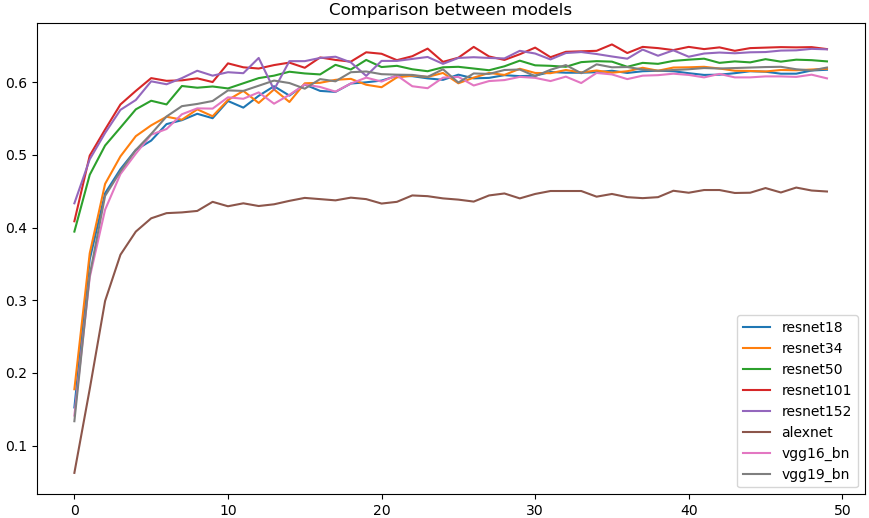
\includegraphics[width = 12 cm]{epoch-accuracy_comparison.png}
        \caption[Comparison between epoch/accuracy for each model]{Comparison between epoch/accuracy for each model. The x axis is the number of epoch, while the y axis is the accuracy achieved}
         \label{fig:com_ep_ac_models}
     \end{figure}
\begin{figure}[h]
\centering 
	    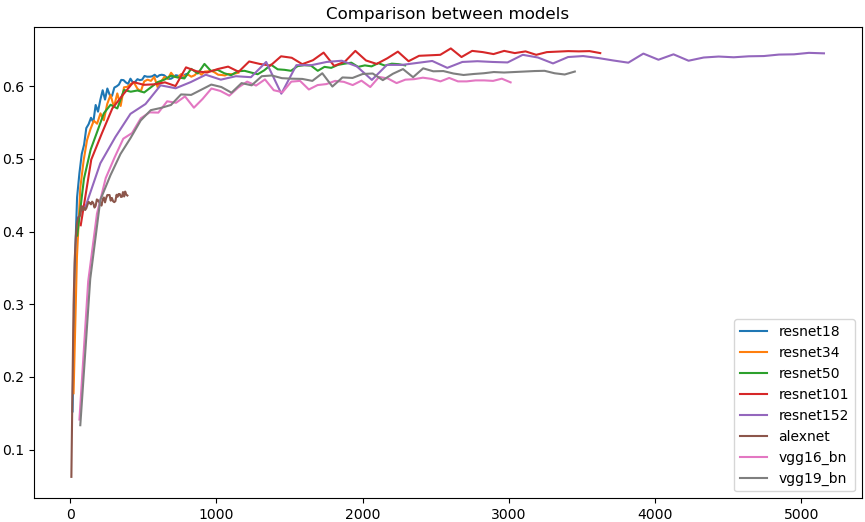
\includegraphics[width = 12 cm]{time-accuracy_comparison.png}
        \caption[Comparison between training time/accuracy for each model]{Comparison between training time/accuracy for each model. The x axis is the training time in seconds, while the y axis is the accuracy achieved}
        \label{fig:com_ti_ac_models}
\end{figure}



As suspected, for each model, the accuracy grows logarithmically higher as the number of  epochs increments, or as the training time increments. A closer inspection of Fig. \ref{fig:com_ti_ac_models} lets us derive other conclusions. Alexnet finishes training in considerably less time compared to the other networks (\textasciitilde 6 minutes), albeit reaching the lowest accuracy overall (45\%). We can observe this difference in time by looking at Fig.\ref{fig:sing_acc_train2} and Fig.\ref{fig:sing_acc_train}, which shows the behaviour of Alexnet, Resnet101, Resnet152 and VGG19 in the same settings. \\
As also shown in the previous graphs, Resnet101 achieved the best overall accuracy at around 65\% with a training time of \textasciitilde 62 minutes, followed by Resnet152, which needed  \textasciitilde 90 minutes to reach an accuracy of \textasciitilde 64\%. Finally, VGG19 took \textasciitilde 60 minutes to reach an accuracy of 61\%. \\
In order to collect more information about the response of the model, we should take a closer look at how they performed individually.\\

\begin{figure}[h]
     \begin{subfigure}{0.5\textwidth}
	    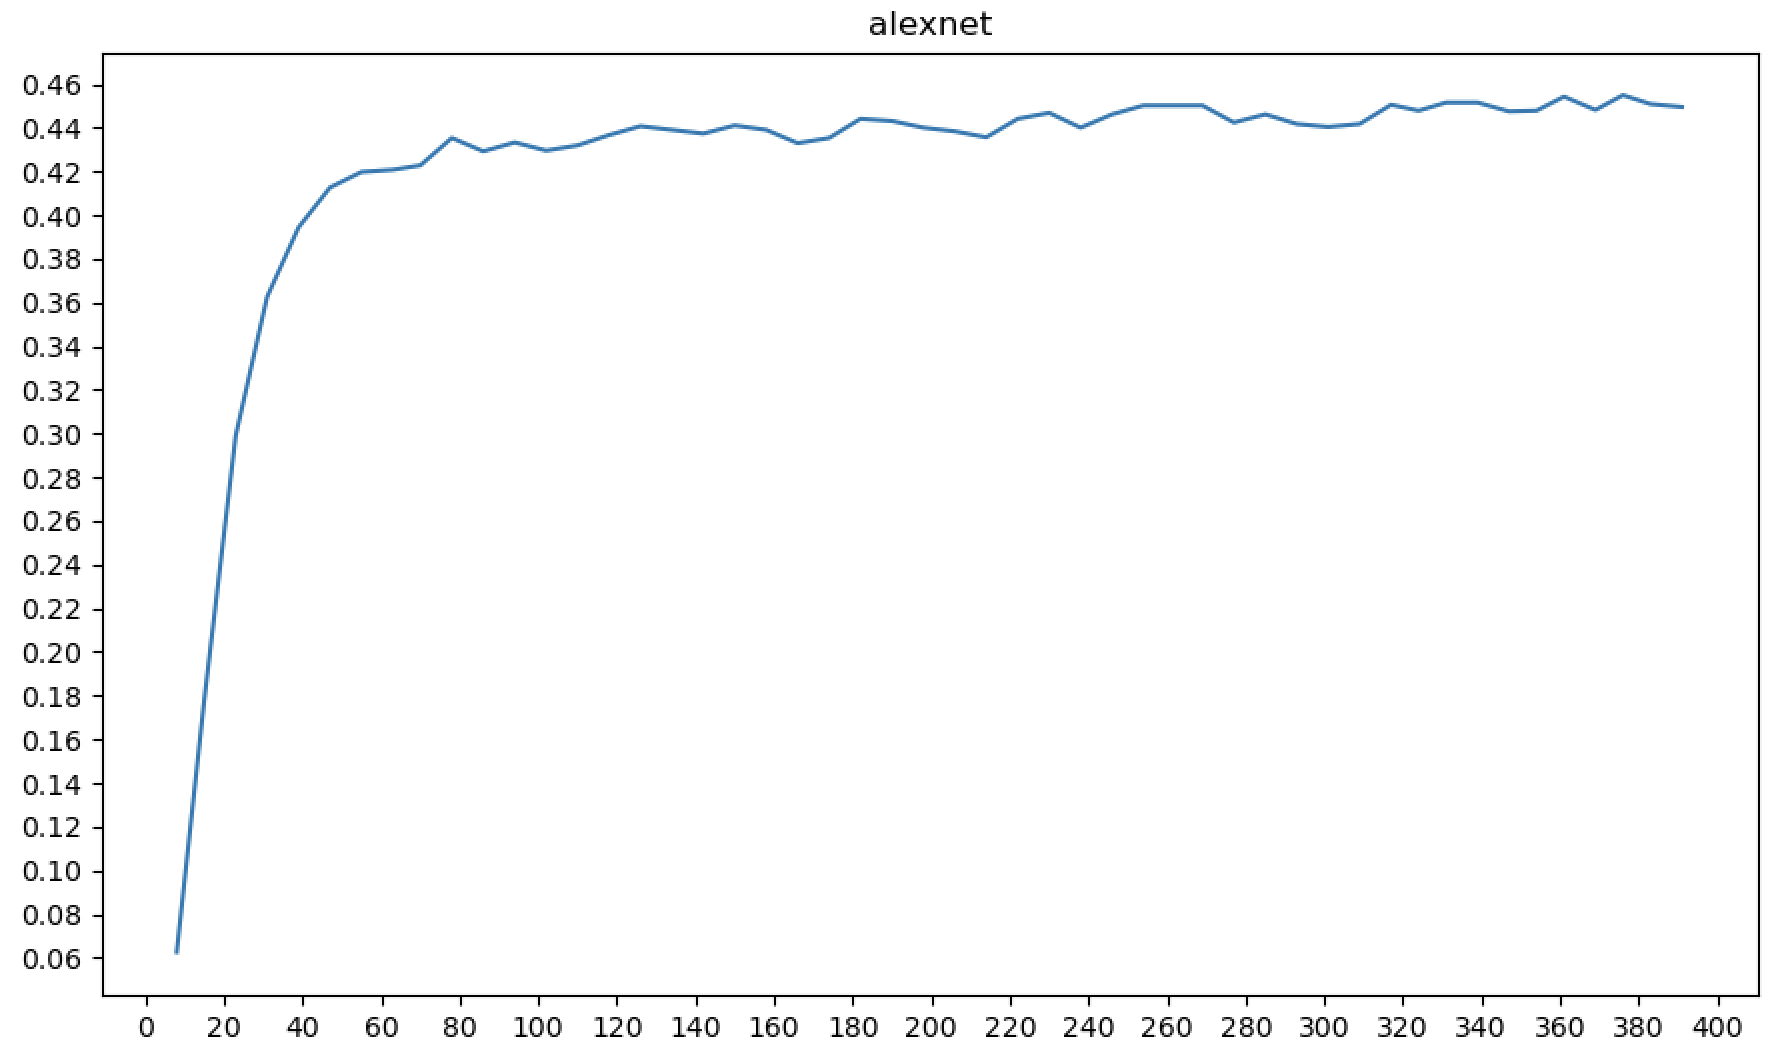
\includegraphics[width = \gws cm]{alexnet_acc_train.png}
         \label{fig:alexnet_acc_train}
     \end{subfigure}
     \hfill
     \begin{subfigure}{0.5\textwidth}
	    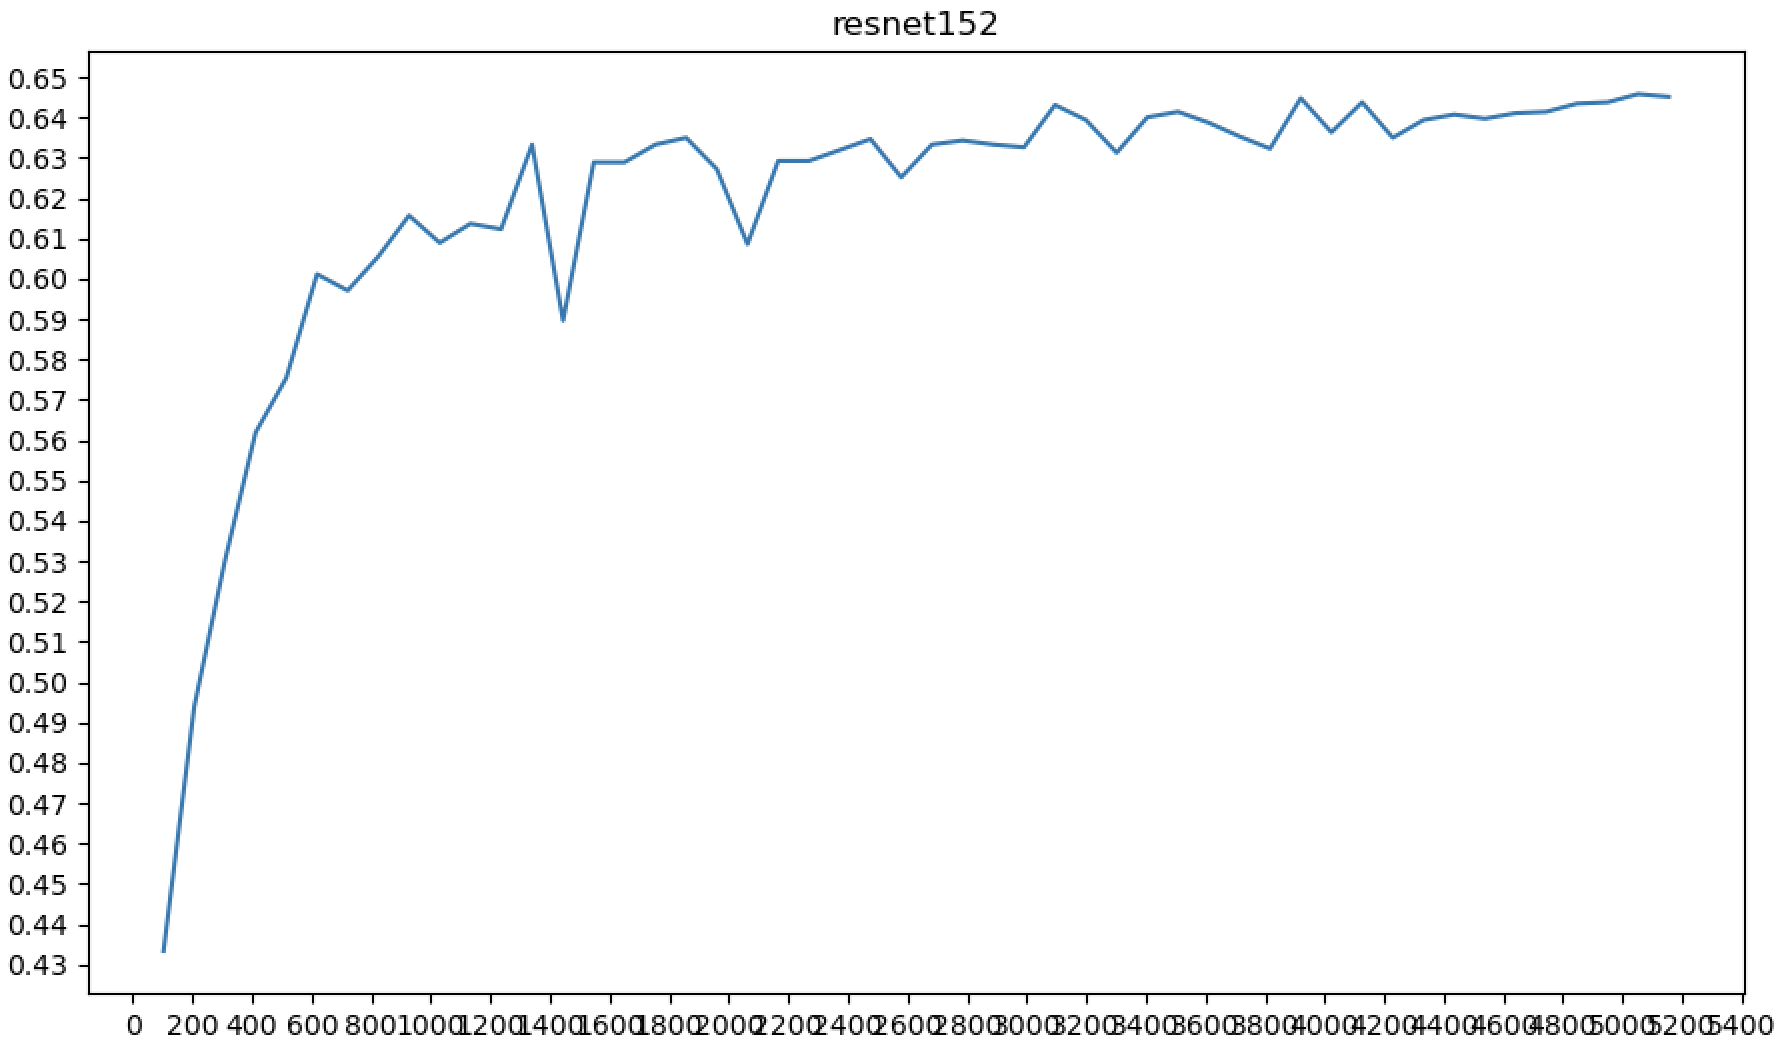
\includegraphics[width = \gws cm]{resnet_152_acc_train.png}
        \label{fig:resnet_152_acc_train}
     \end{subfigure}\\
     \caption{Accuracy of Alexnet and Resnet152 against training time in seconds}
        \label{fig:sing_acc_train2}
\end{figure}
\begin{figure}[h]
     \begin{subfigure}{0.5\textwidth}
	    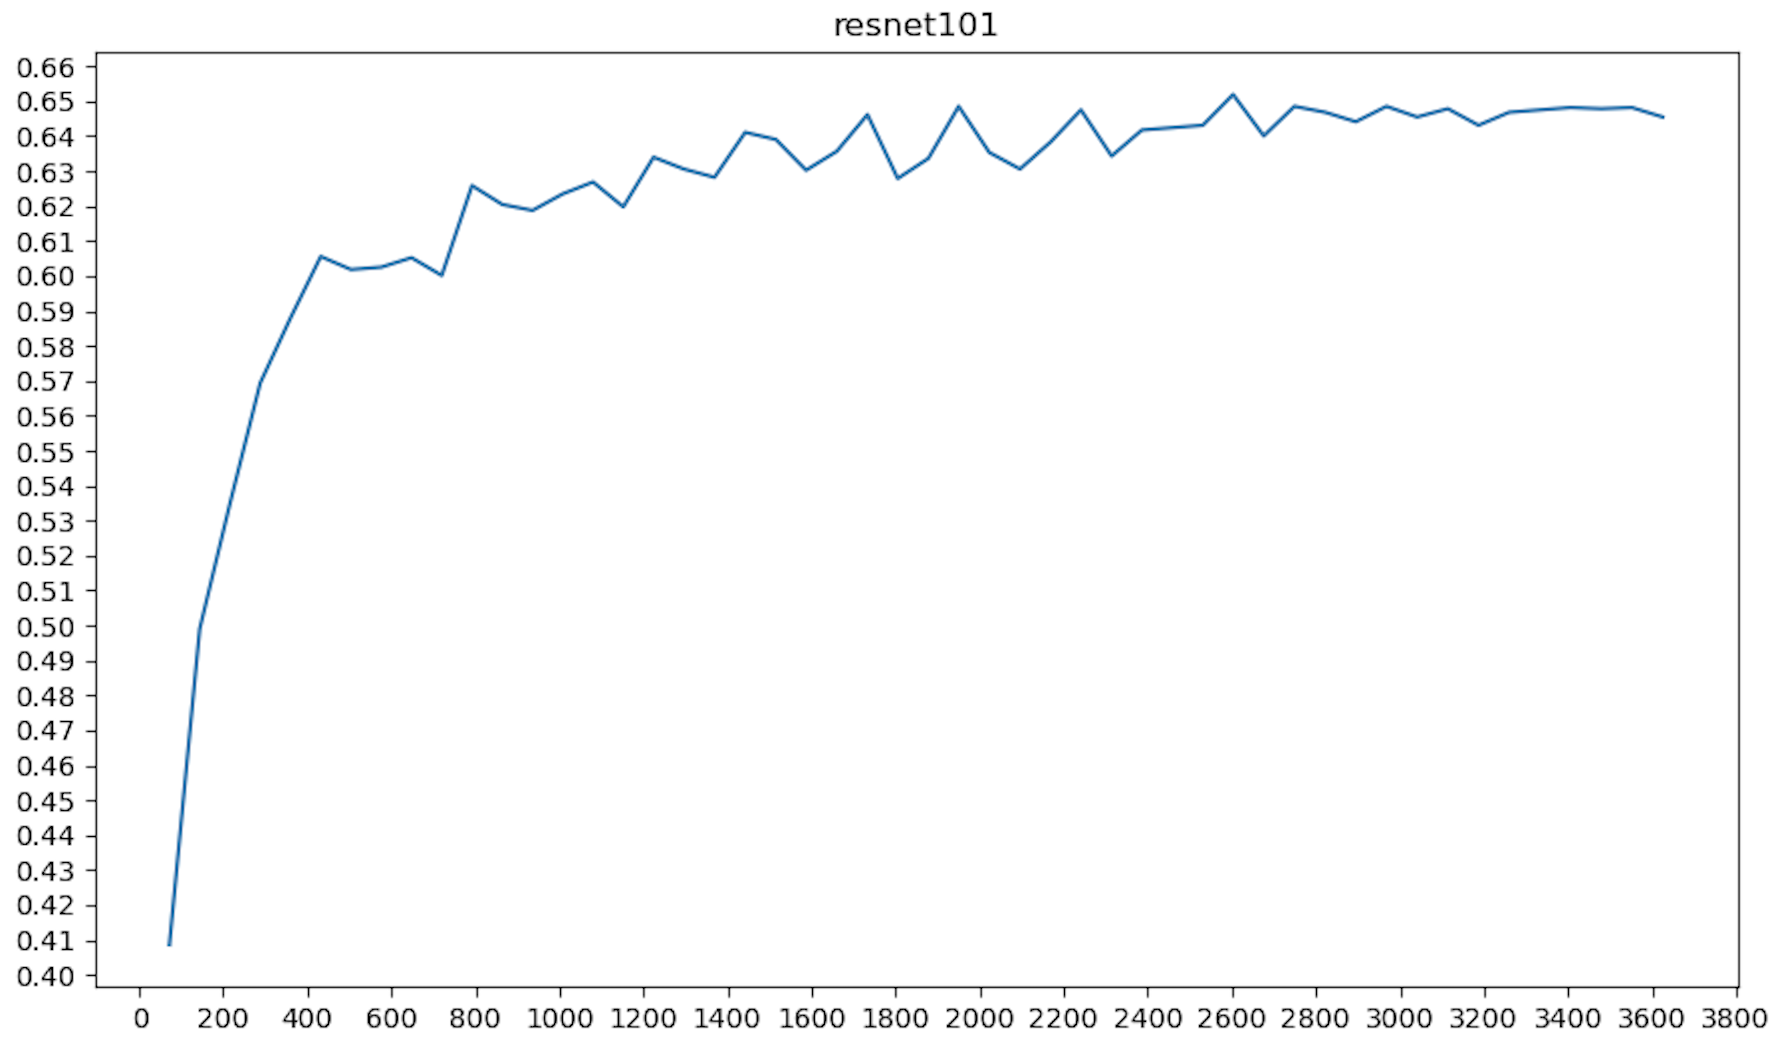
\includegraphics[width = \gws cm]{resnet_101_acc_train.png}
        \label{fig:resnet_1o1_acc_train}
     \end{subfigure}
     \begin{subfigure}{0.5\textwidth}
	    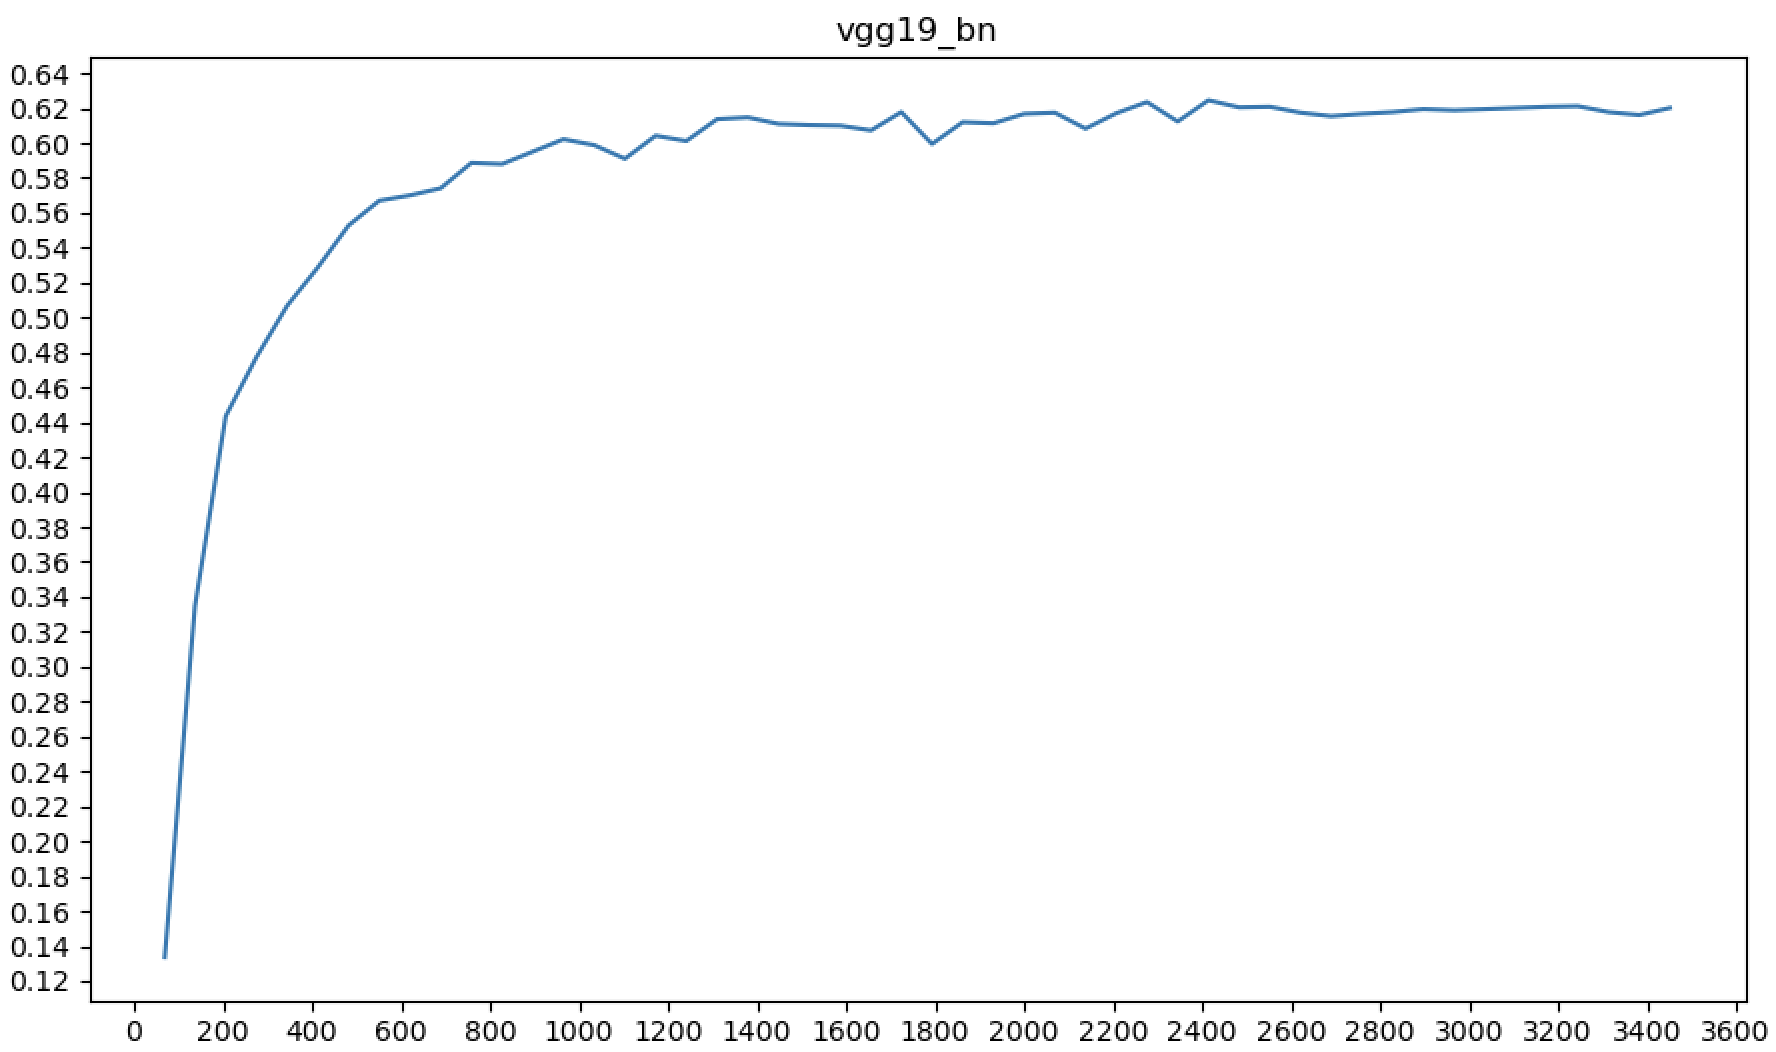
\includegraphics[width = \gws cm]{vgg_19_acc_train.png}
        \label{fig:vgg_19_acc_train}
     \end{subfigure}
        \caption{Accuracy of Resnet101 and VGG9 against training time in seconds}
        \label{fig:sing_acc_train}
\end{figure}
Fig.\ref{fig:sing_acc_train2} and Fig.\ref{fig:sing_acc_train} also show how stable each model was during training. The stability we are observing, in this instance, is how fluctuating each model has been during training, regarding its accuracy. The less fluctuating it is, the better we able to predict the accuracy from the training time, or the number of epochs, and vice-versa. From the results, we can see that Resnet152 and Resnet101 tend to fluctuate more compared to Alexnet or VGG19 (Fig. \ref{fig:sing_acc_train}). \\
Such fluctuation, however, does not hide a trend which is common amongst all models: after a certain number of epochs, the accuracy tends to stabilise and grow significantly slower. Fig. \ref{fig:com_ep_ac_models} can help us locate the point at which the accuracy stops increasing at a high rate at around 10 epochs and this is further proved by Fig. \ref{fig:sing_acc_ep}.\\
\begin{figure}[h]
     \begin{subfigure}{0.5\textwidth}
	    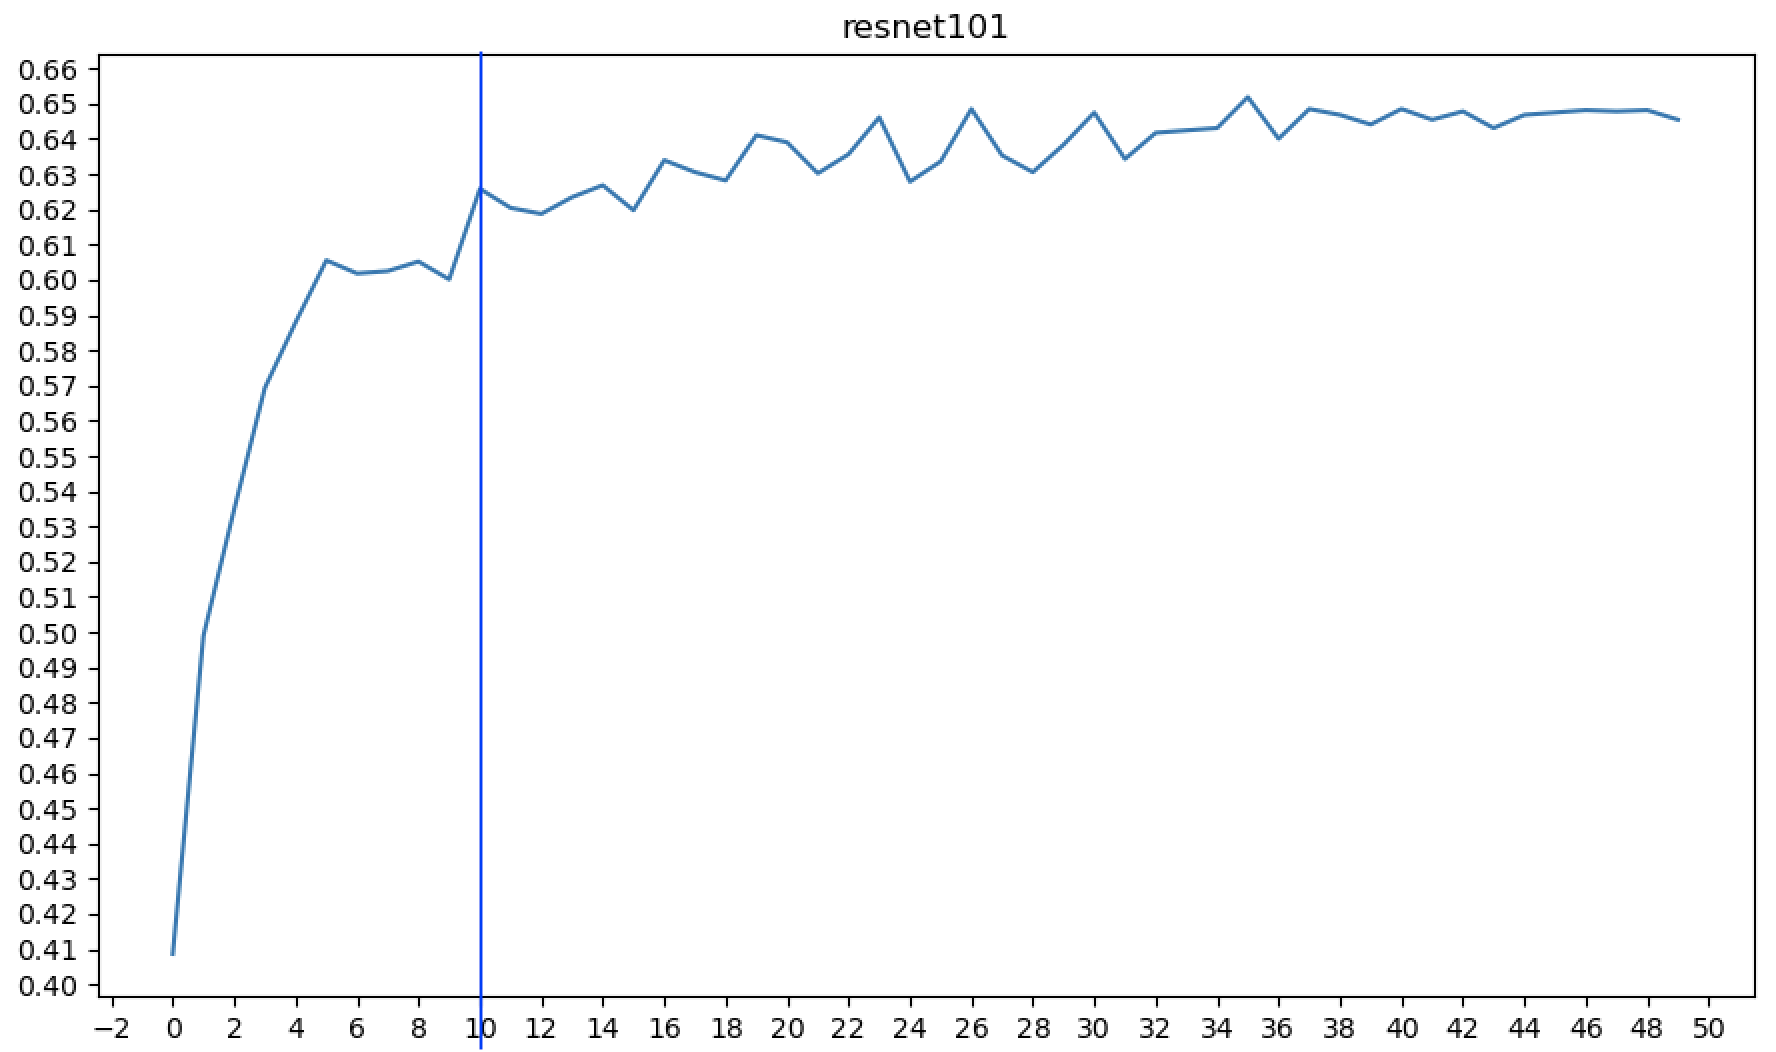
\includegraphics[width = \gws cm]{resnet_101_acc_ep.png}
        \label{fig:resnet_101_acc_ep}
     \end{subfigure}
     \begin{subfigure}{0.5\textwidth}
	    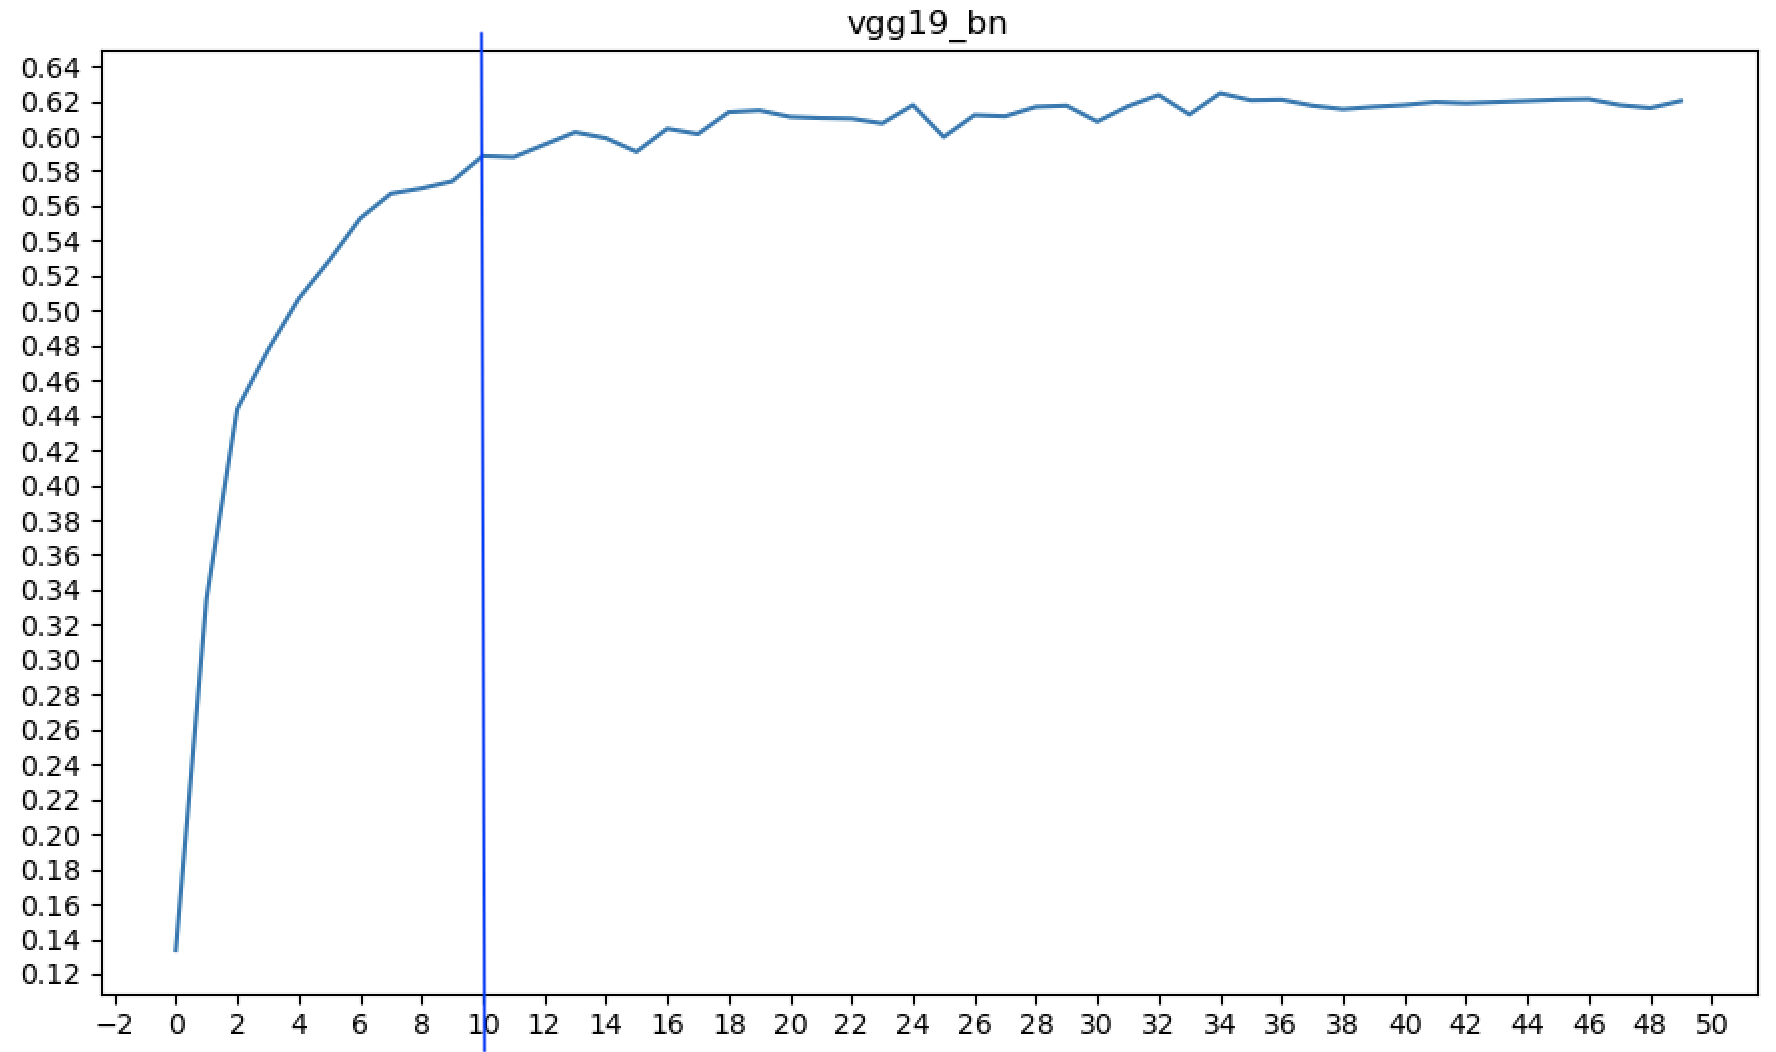
\includegraphics[width = \gws cm]{vgg_19_acc_ep.png}
        \label{fig:vgg_19_acc_ep}
     \end{subfigure}
        \caption{Breaking point of Resnet101 and VGG19}
        \label{fig:sing_acc_ep}
\end{figure}\\



We can further analyse the behaviour of each model for the first 10 epochs by observing Fig. \ref{fig:acc_training_10}. This graph gives us a closer look at how the models have been trained and how the curve looks like. Differently from the previous graph, Resnet152 this time reached a higher accuracy, however it was also the model that took the most time to fully complete the training.\\
On the other hand, from Fig. \ref{fig:acc_training_10}, we can clearly observe  that, if compared with each other for the same training time, shallower networks like Resnet34 or Resnet50 achieved higher accuracy than deeper networks like Resnet152. This is obviously due to the fact that, within the same training time, shallower networks manage to complete more epochs, and therefore complete more training cycles. As a matter of fact, if we were to compare models on an epoch base we will find that deeper networks will achieve better accuracy when given the same number of epochs. \\
If we observe Fig. \ref{fig:com_ti_ac_models} before the 1000 seconds mark, we can see that Resnet18's curve starts to flatten, reaching an accuracy of \textasciitilde 61\%, while the others tend to reach smaller accuracy values. Around the 1000 seconds mark the behaviour of all the models starts to equalise and afterwards the accuracy of deeper networks will increase reaching higher values. As mentioned previously, this is due to the models being able to finish more epochs within the same time frame. In this case, the models reached to finish the training completely, as shown in \ref{fig:com_ti_ac_models}. 
Models from different architectures do not follow this trend. Alexnet, as we already discussed above, does not manage to reach somewhat close to the same accuracy of the other models. VGG16 and VGG19 follow similar trends and both curves overlap multiple times.  Even though VGG19 is considerably bigger than VGG16 (\cite{simonyan2015deep}), they reach very similar accuracy even before the 1000 seconds marks with very similar training time. \\
\begin{figure}[h]
       \centering 
	    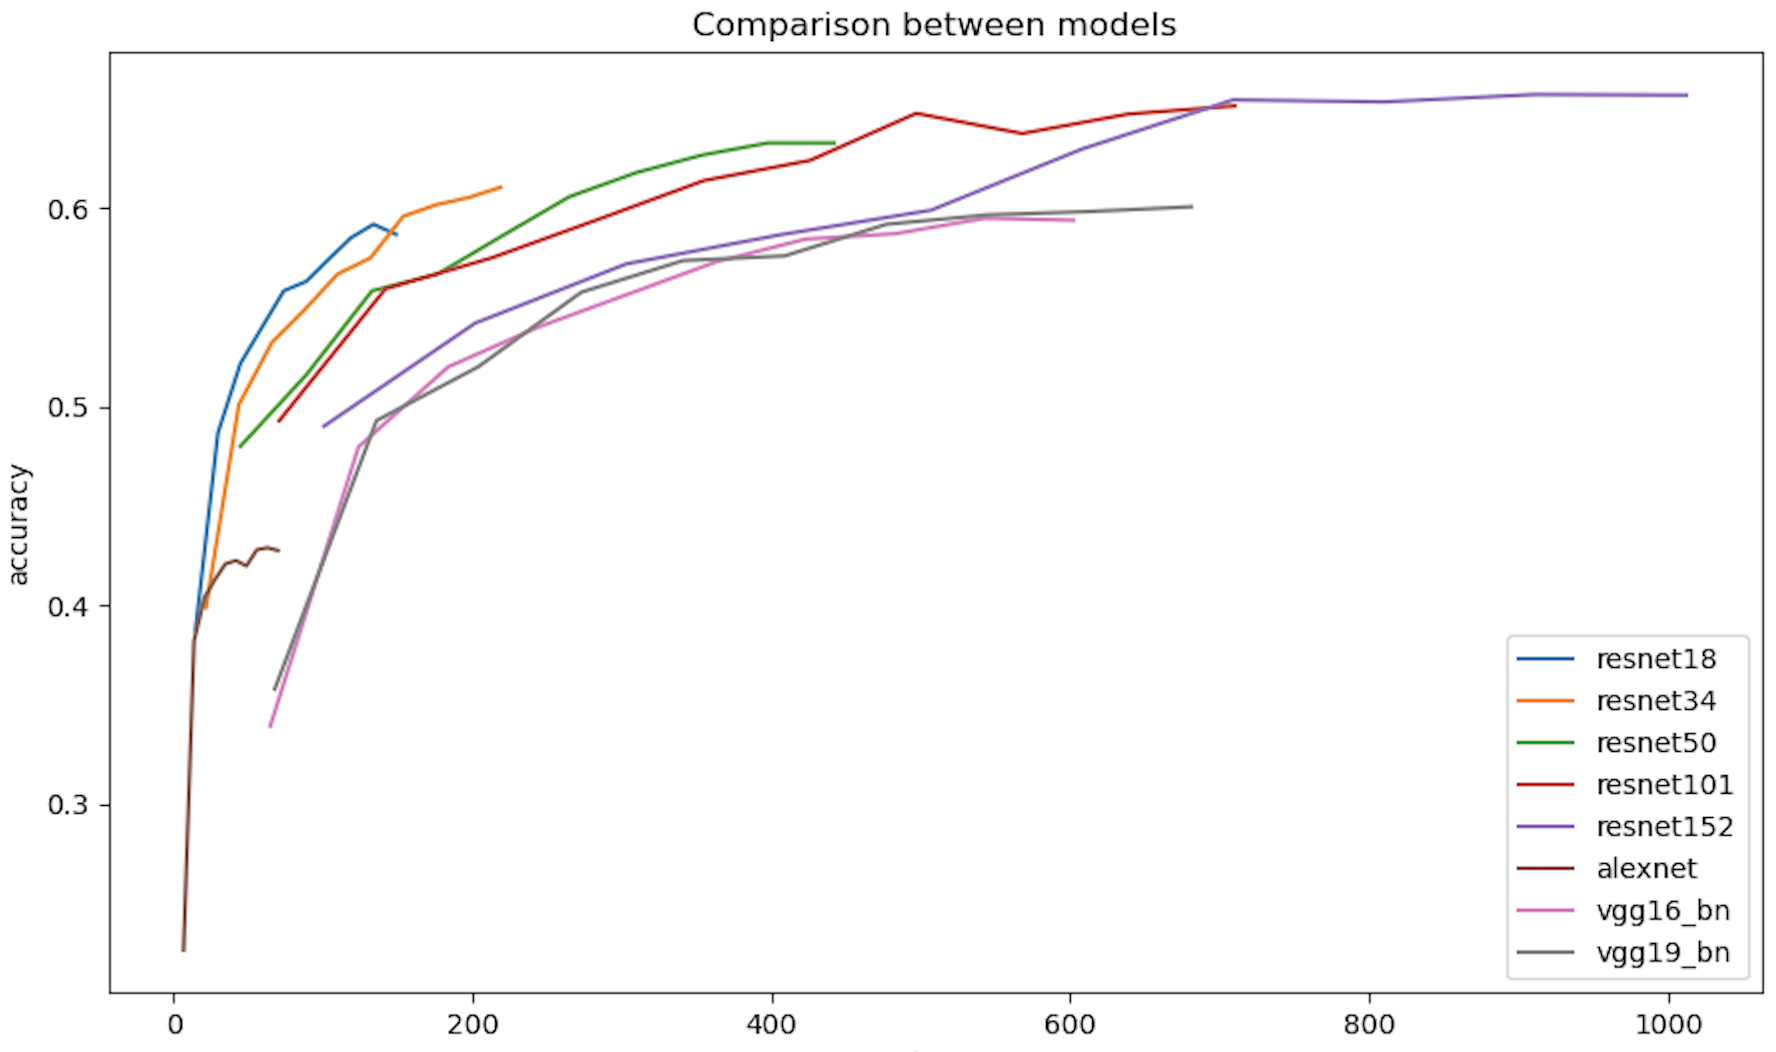
\includegraphics[width = 12 cm]{acc_training_time_10.png}
        \caption[Comparison between training time and accuracy for each model for 10 epochs]{Comparison between training time and accuracy for each model for 10 epochs. The x axis is the training time in seconds, while the y axis is the accuracy achieved}
         \label{fig:acc_training_10}
\end{figure}


\begin{figure}[h]
       \centering 
	    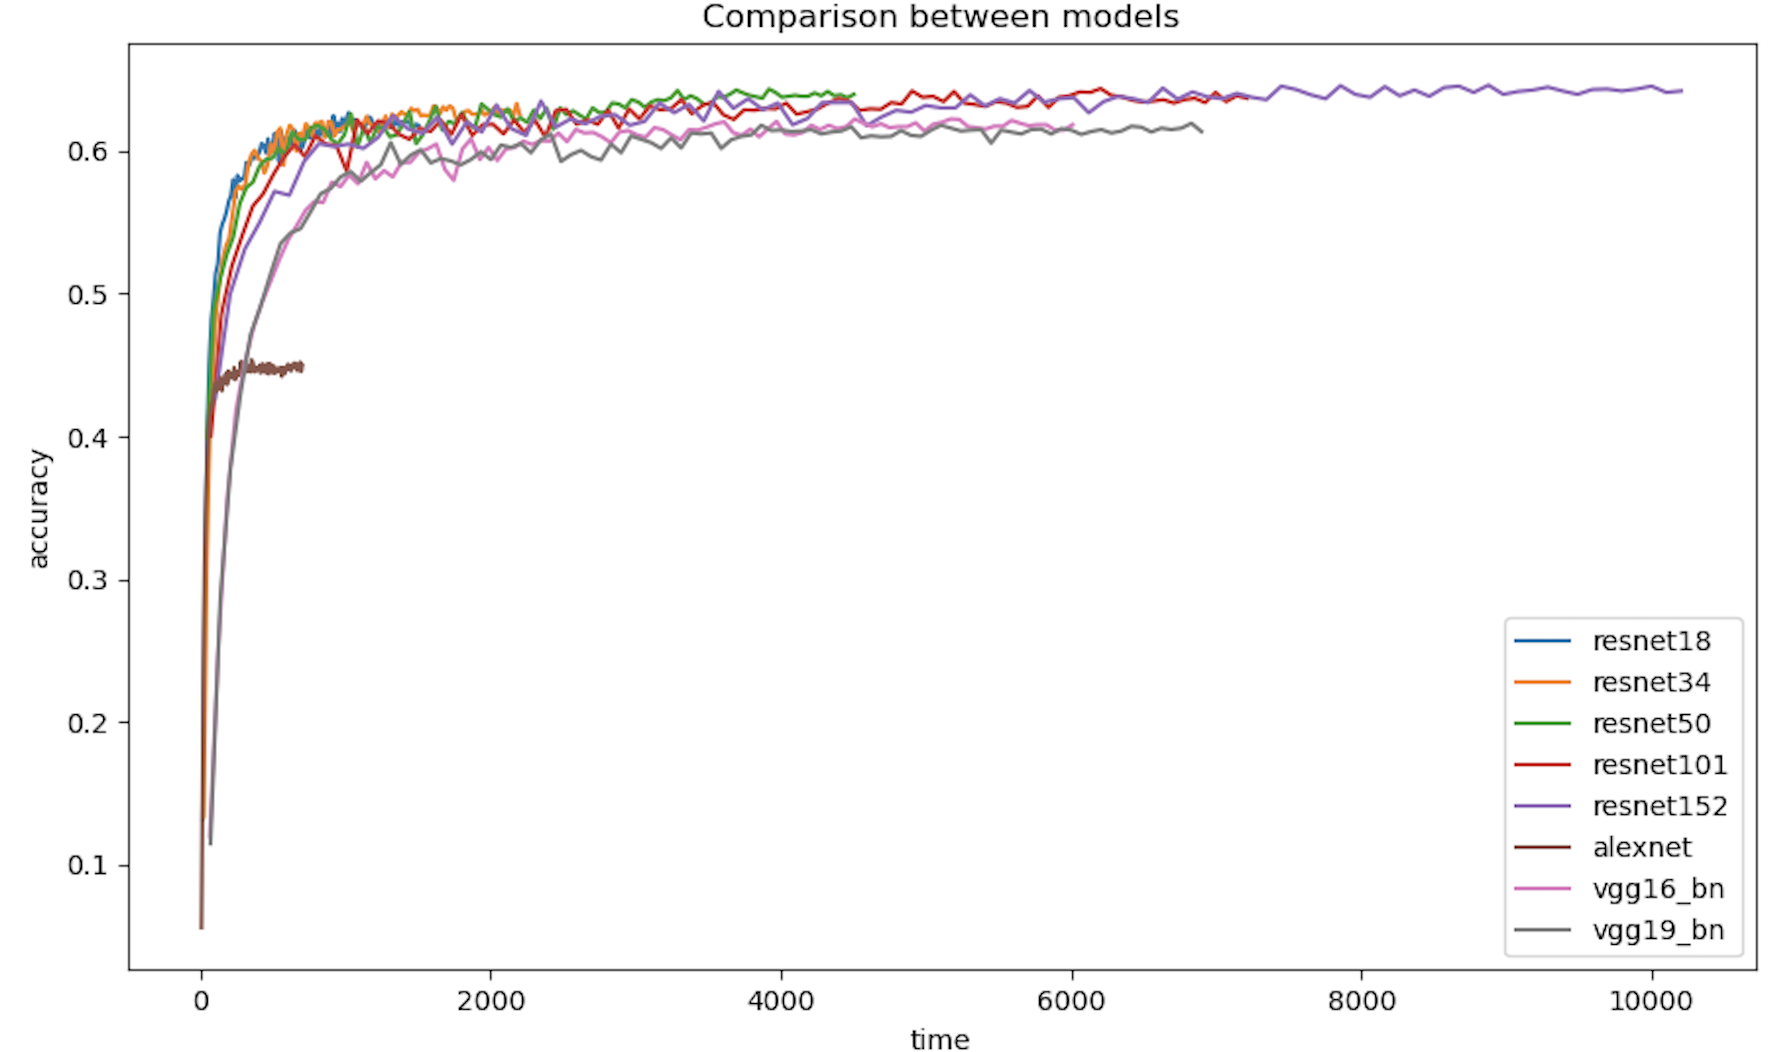
\includegraphics[width = 12 cm]{time_acc_100.png}
        \caption[Comparison between training time and accuracy for each model for 100 epochs]{Comparison between training time and accuracy for each model trained for 100 epochs. The x axis is the training time in seconds, while the y axis is the accuracy achieved}
         \label{fig:time_acc_100}
\end{figure}




This behaviour is further highlighted in Fig. \ref{fig:time_acc_100} which shows the behaviour of the models trained for 100 epochs. We can see that once again around 1000 seconds the curve of every model starts to flatten and the models using the Resnet architectures achieve similar accuracy. The highest accuracy is achieved by Resnet152, which also needed the most training time. Surprisingly, Resnet50 performed better than Resnet101, achieving better accuracy with less training time.
VGG16 and VGG19 performed similarly, displaying overlapping curves, with VGG19 once again requiring more training time. \\
More importantly, however,this graph confirms the results and the hypothesis we made previously. Furthermore, we can use all the data we acquired to calculate the average training time required for each epoch. The results are provided in table \ref{tab:time_f_epoch}.
\begin{table}[h]
\centering
\begin{tabular}{ p{2cm} p{2cm}   }
 Model&Time (s)\\
 \hline
Resnet18&15.01\\
Resnet34&22.0\\
Resnet50&45.02\\
Resnet101&72.11\\
Resnet152&102.02\\
Alexnet&7.01\\
VGG16&60.09\\
VGG19&68.97\\
 \hline
\end{tabular}
\caption{Average time for each epoch}
\label{tab:time_f_epoch}
\end{table}

Comparing the training results we just obtained with the ones obtained for the 'plant\_seedlings\_v2' dataset, we can see that, regardless of the raw values we obtained, the models behaved equivalently in training. \\
Training for 100 epochs also gives us more complete insights regarding the future performance of our models. In other words, we can determine when the model starts to over-fit or under-fit and when to stop the training to avoid future poor performances. \\
\begin{figure}[h]
\begin{subfigure}{0.5\textwidth}
	    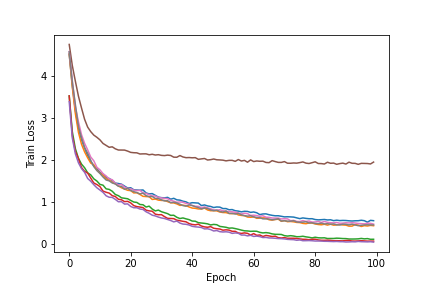
\includegraphics[width = \gws cm]{epoch_train_loss.png}
	    \caption{Training Loss calculated over 100 epochs}
        \label{fig:train_loss}
        
     \end{subfigure} \hfill
     \begin{subfigure}{0.5\textwidth}
	    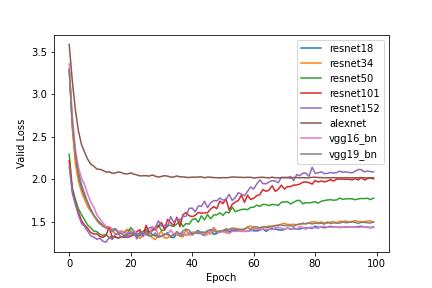
\includegraphics[width = \gws cm]{epoch_valid_loss.png}
	    \caption{Validity Loss calculated over 100 epochs}
         \label{fig:valid_loss}
         
     \end{subfigure}
    
     
     \caption{ Training loss and validity loss of all models calculated over 100 epochs}
        \label{fig:tran_valid_loss}
\end{figure}


As shown in Fig. \ref{fig:train_loss}, the train loss decreases at each epoch for each model. For Alexnet, the curve tends to flatten at around 15 epochs, while for the others it flattens at around 60. Rather than observing the training loss trend alone, however, which does not give us the possibility to comprehend correctly the response of the models, we should compare it to the trend of the validation loss shown in Fig. \ref{fig:valid_loss}. Alexnet remained stable for the duration of the training, with a validation loss comparable to the training loss. The other models, on the other hand, show a rather different behaviour. At around 20 epochs, the validation loss of deeper networks, i.e. Resnet152, Resnet101 and VGG19 starts to increment drastically. For shallower networks of the Resnet architecture, i.e. Resnet18, Resnet34 and Resnet50, and for VGG16 the validation loss decreased for the first 15 epochs and started to increment only after \textasciitilde40.\\
In section n. \ref{sec:of_uf} we defined over-fitting to be a situation in which the validation loss is much larger than training and from Fig. \ref{fig:valid_loss} we can see that, although after various numbers of epochs, most of the networks start to enter this condition as the validation loss increases and it becomes much larger than their training loss. We also discussed some techniques to avoid this, like for e.g. Cross-Validation. For the purpose of this experiment, we only split the dataset 80-20, hence we used no cross-validation or augmentation on the data-set whatsoever. \\
In this analysis, we can observe the first difference with the results obtained in the first experiment. First of all, the training loss decreases rather slowly when compared to Fig. \ref{fig:tran_valid_loss_seeds_res_100} or Fig.  \ref{fig:tran_valid_loss_seeds_res_100_2}. The validation loss, on the other hand, as we already noticed, increased as the training time increased, while for the other experiment it either remained stable, or increased minimally.
To measure inference time, we need to collect a dataset of related pictures, which are not part of the training dataset, to feed to each model. For our tests, we are going to use a data set composed of 200 random pictures. The pictures we are going to use are going to be of different dimensions and different quality in order to see if we can recognize patterns. We can see the results in Fig. \ref{fig:inf_time_epoch_c}, which displays the training time in milliseconds graphed against the accuracy and the number of epoch used to train. From this figure, we can clearly see that the inference time for every model rarely is measured to be more than 230 milliseconds, with the exception of a few outliers, and most of the models for most epochs have an accuracy between 87\% and 92\%. In addition, if we analyse the inference time based on the number of epochs (Fig. \ref{fig:inf_time_epoch}) the models display similar responses.  \\


\begin{figure}[h]
     \begin{subfigure}{0.5\textwidth}
	    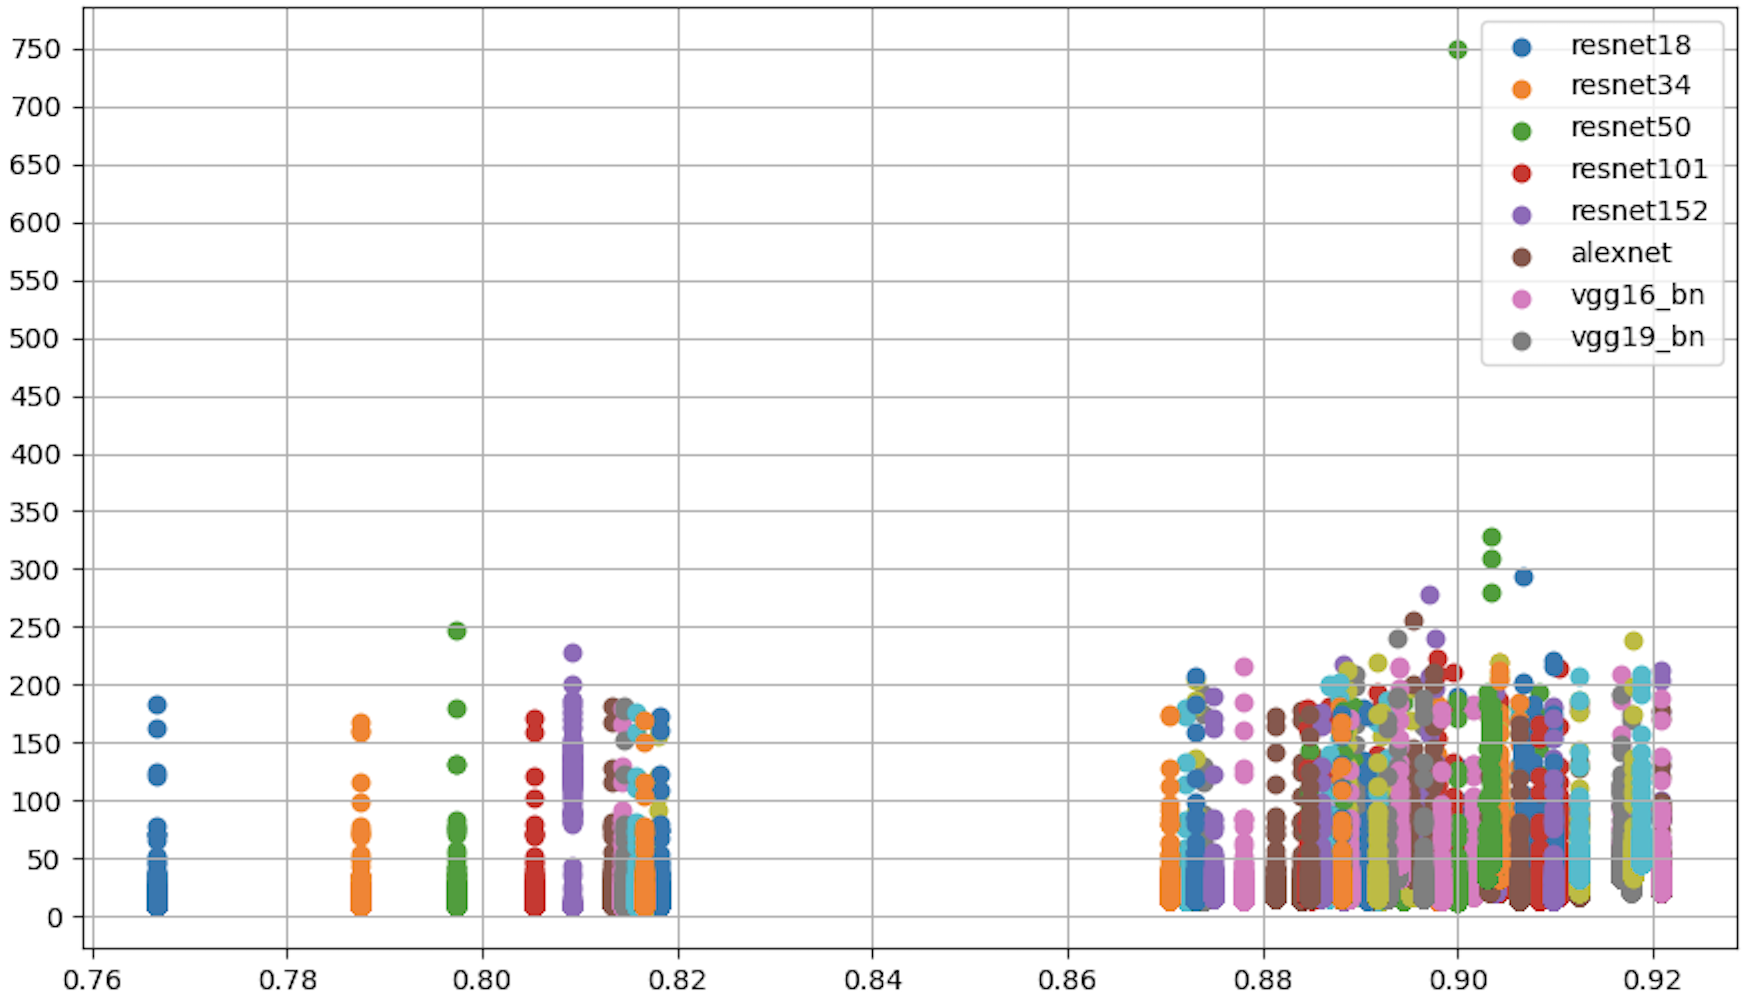
\includegraphics[width = \gws cm]{inf_time_accuracy.png}
	    \caption{}
         \label{fig:inf_time_accuracy}
     \end{subfigure}
     \hfill
     \begin{subfigure}{0.5\textwidth}
	    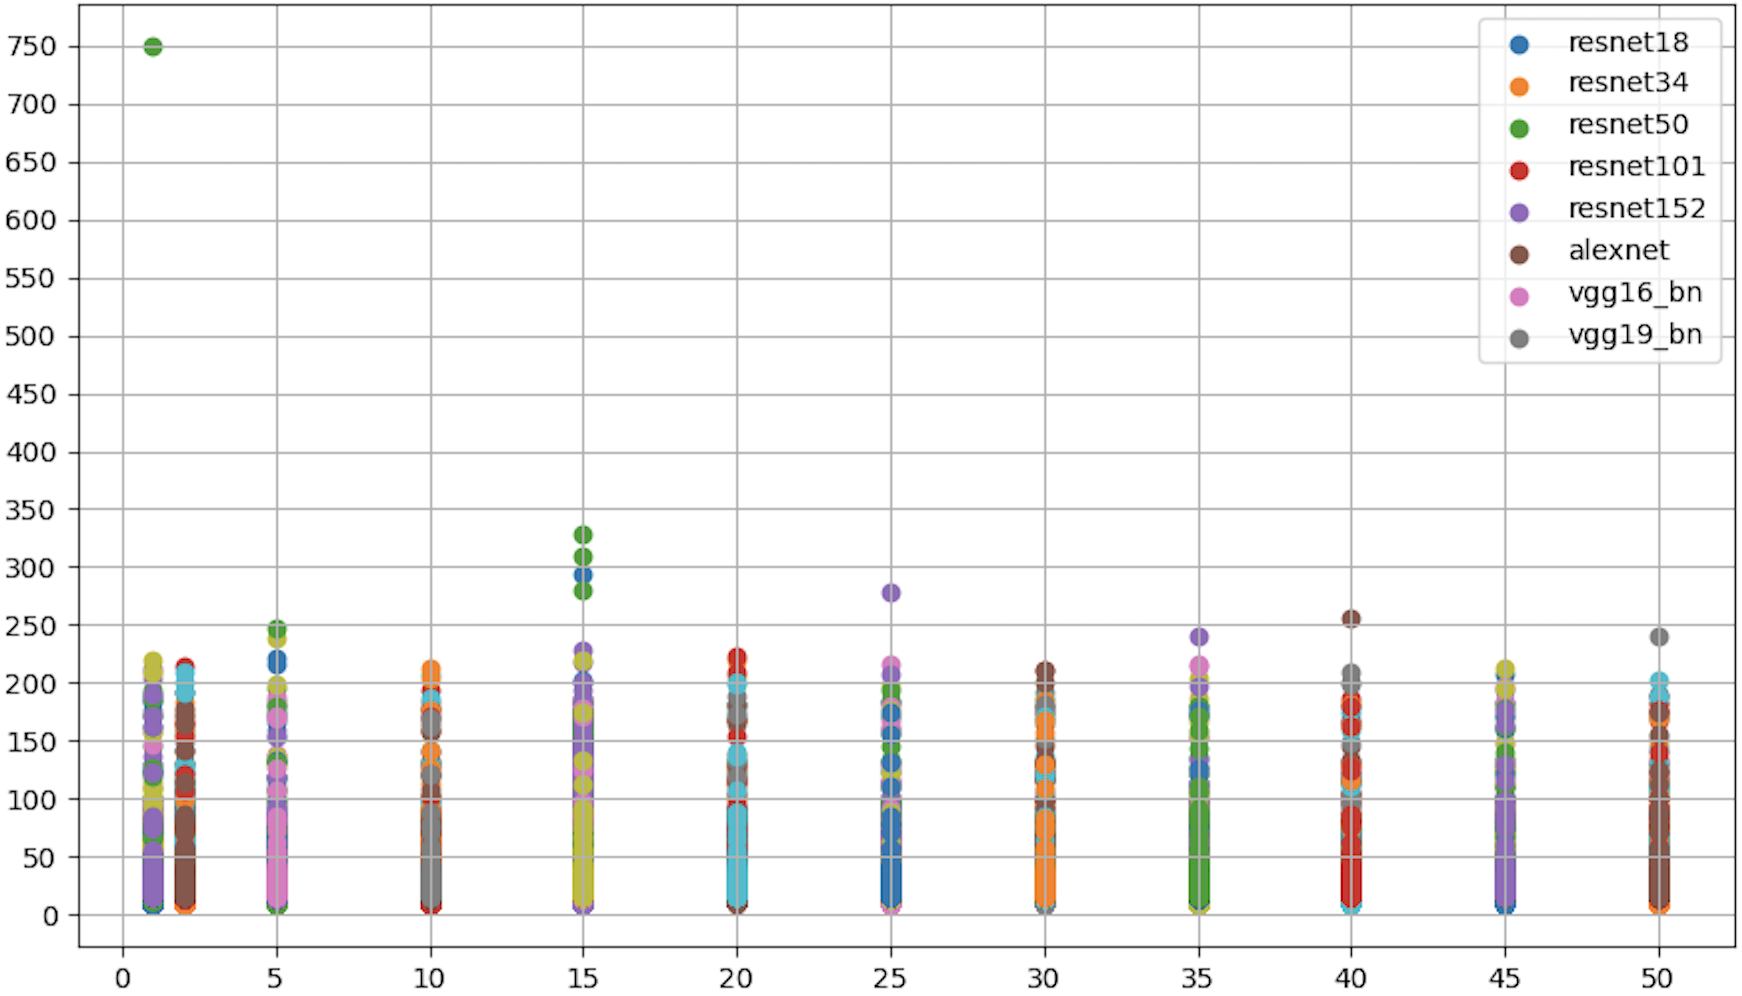
\includegraphics[width = \gws cm]{inf_time_epoch.png}
	    \caption{}
        \label{fig:inf_time_epoch}
     \end{subfigure}\\
     \caption[Inference time measured for each model]{Inference time measured for each model using the 200 pictures dataset discussed previously. The inference time is in milliseconds, while the accuracy for Fig. \ref{fig:inf_time_accuracy}is the percentage of correct predictions.}
        \label{fig:inf_time_epoch_c}
\end{figure}

\begin{figure}[h]
     \begin{subfigure}{0.5\textwidth}
	    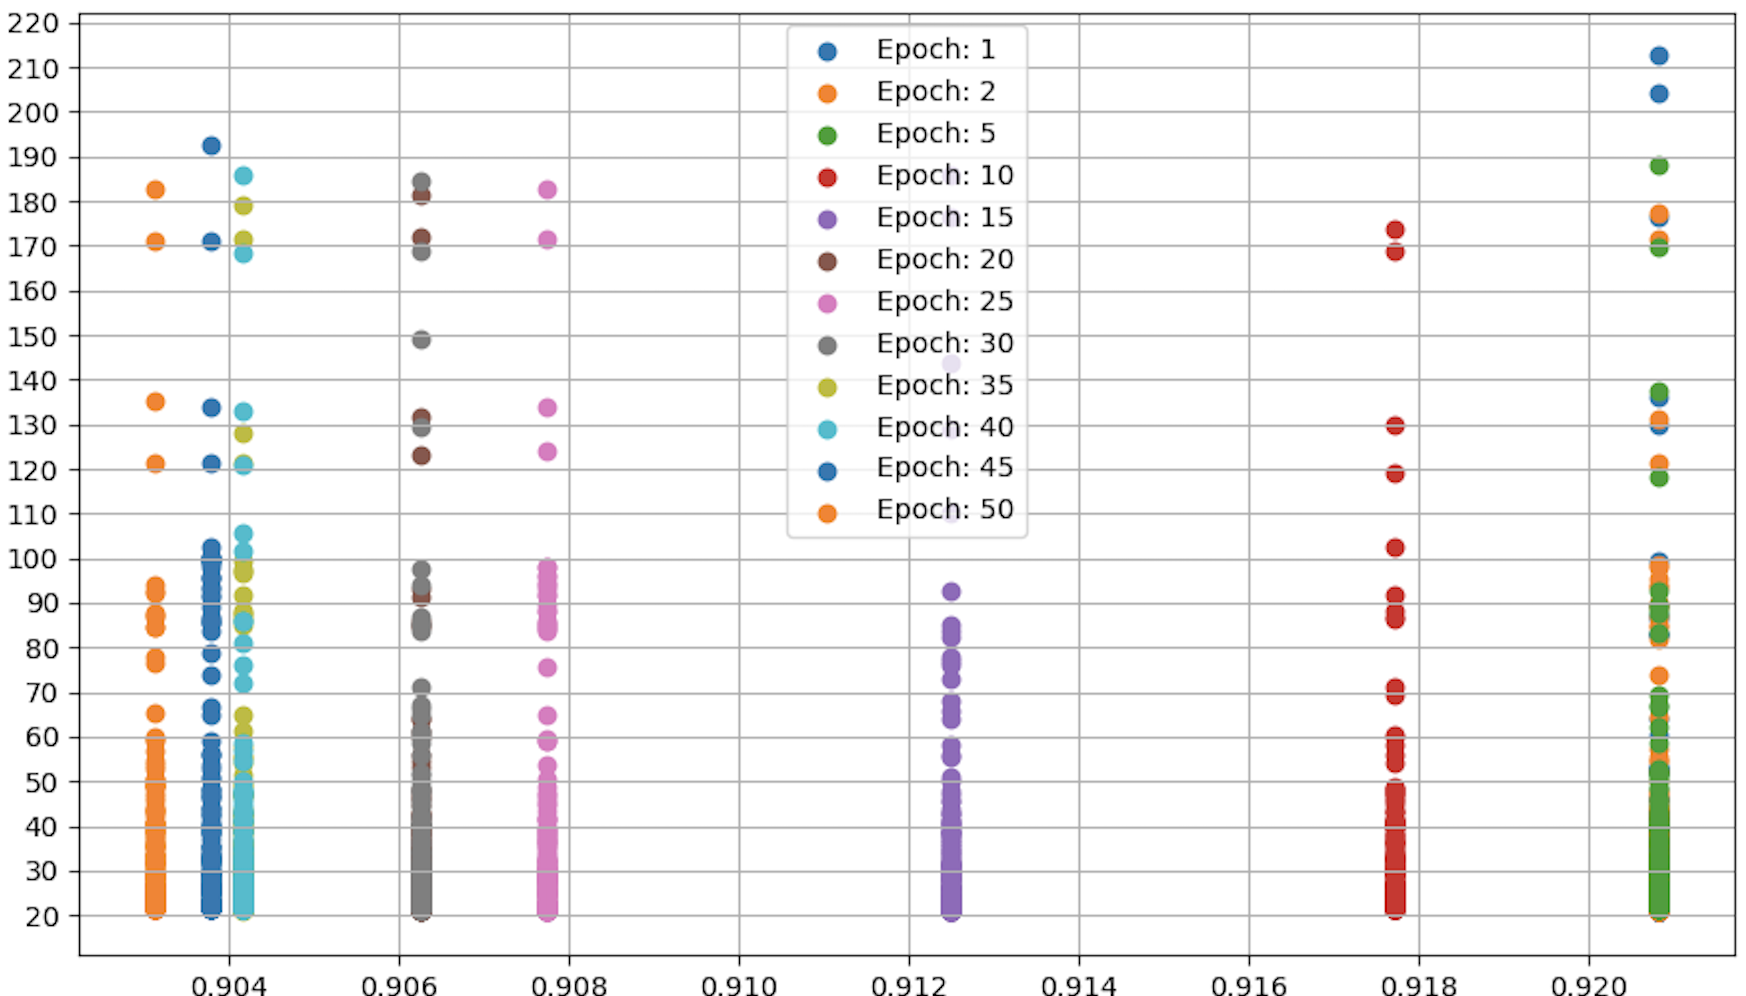
\includegraphics[width = \gws cm]{inf_acc_resnet18.png}
	    \caption{Resnet18}
         \label{fig:inf_acc_resnet18}
         
     \end{subfigure}
     \hfill
     \begin{subfigure}{0.5\textwidth}
	    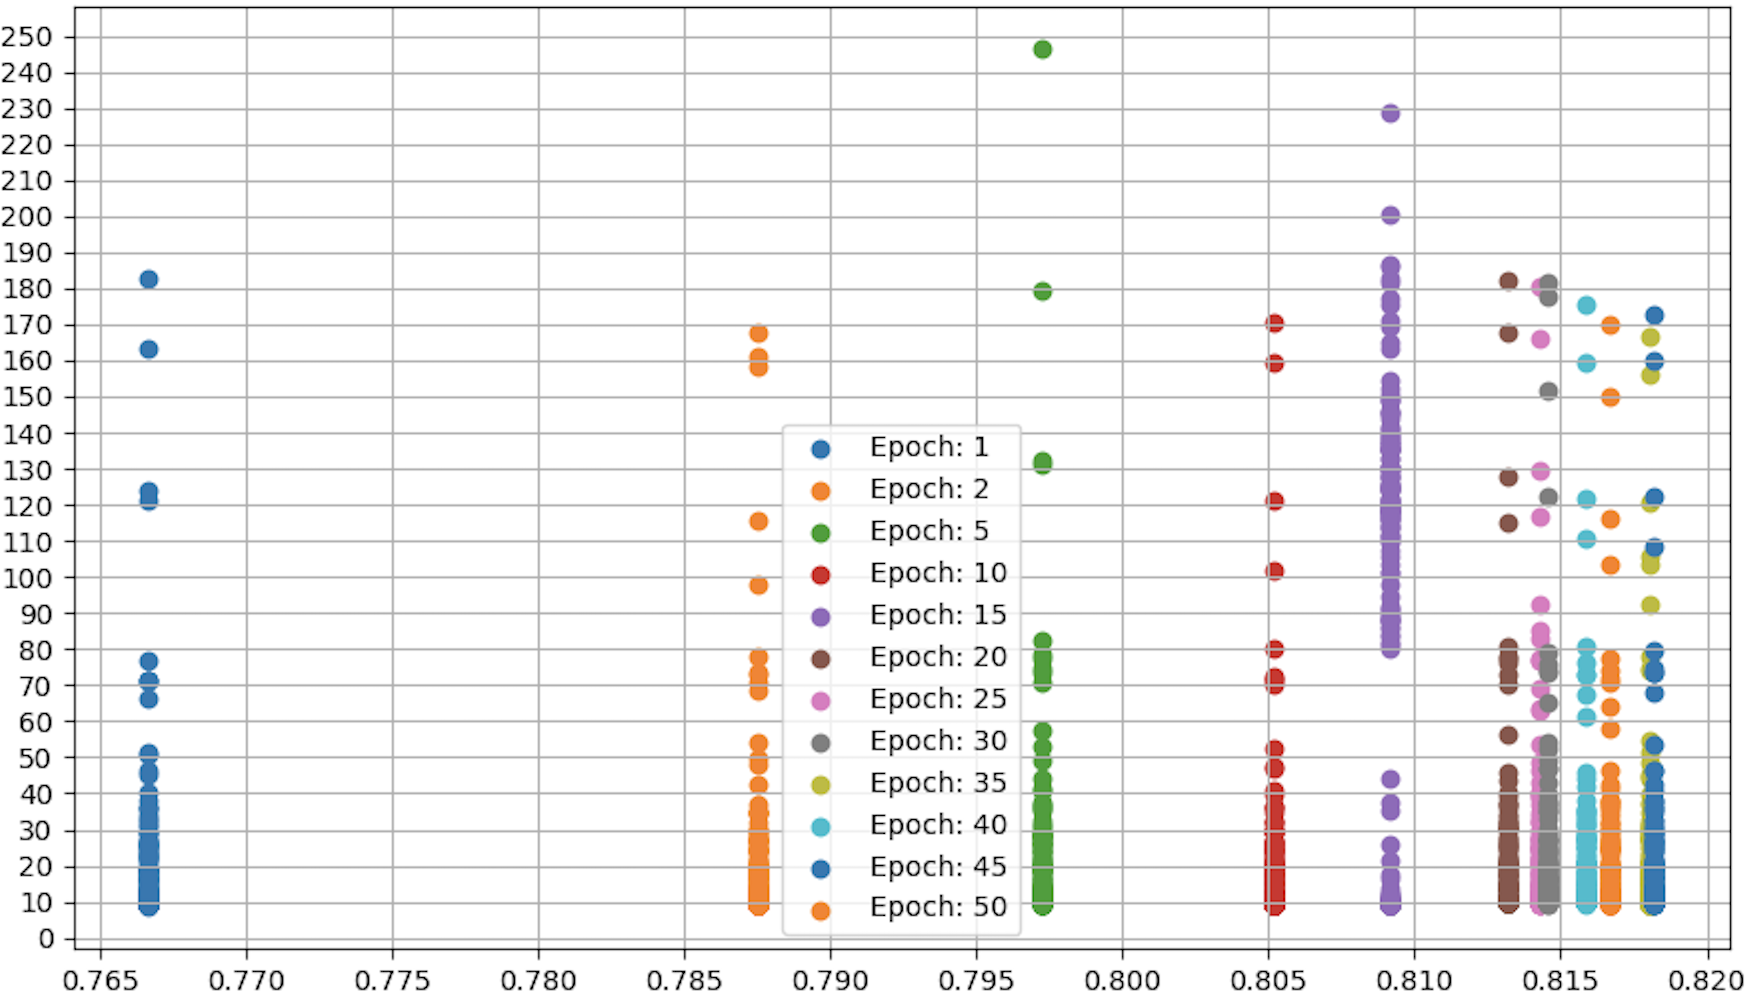
\includegraphics[width = \gws cm]{inf_acc_alexnet.png}
	    \caption{Alexnet}
        \label{fig:inf_acc_alexnet}
        
     \end{subfigure}\\
     \caption{Inference time measured for model Resnet18 and Alexnet}
        \label{fig:inf_acc_c}
\end{figure}
When we compare models individually like in Fig. \ref{fig:inf_acc_c}, other similarities appear. As a matter of fact, when we analyse each model, we can observe that some pictures require considerably more time than others. For example, Fig. \ref{fig:inf_acc_c} shows the measurements obtained by model Resnet18 (\ref{fig:inf_acc_resnet18}) and Alexnet (\ref{fig:inf_acc_alexnet}) and from their response it appears that, at each epoch, there is a constant number of images which takes more time to be processed. \\
We can run the tool once again to identify the 10 images that took more time to be processed at each epoch, in order to analyse them and find elements which can explain such differences. \\
The first property of the image we are going to take a look at is the size of the images. Fig. \ref{fig:size_inference_time_compared} shows the results obtained for each model. 


\begin{figure}[h]
       \centering 
	    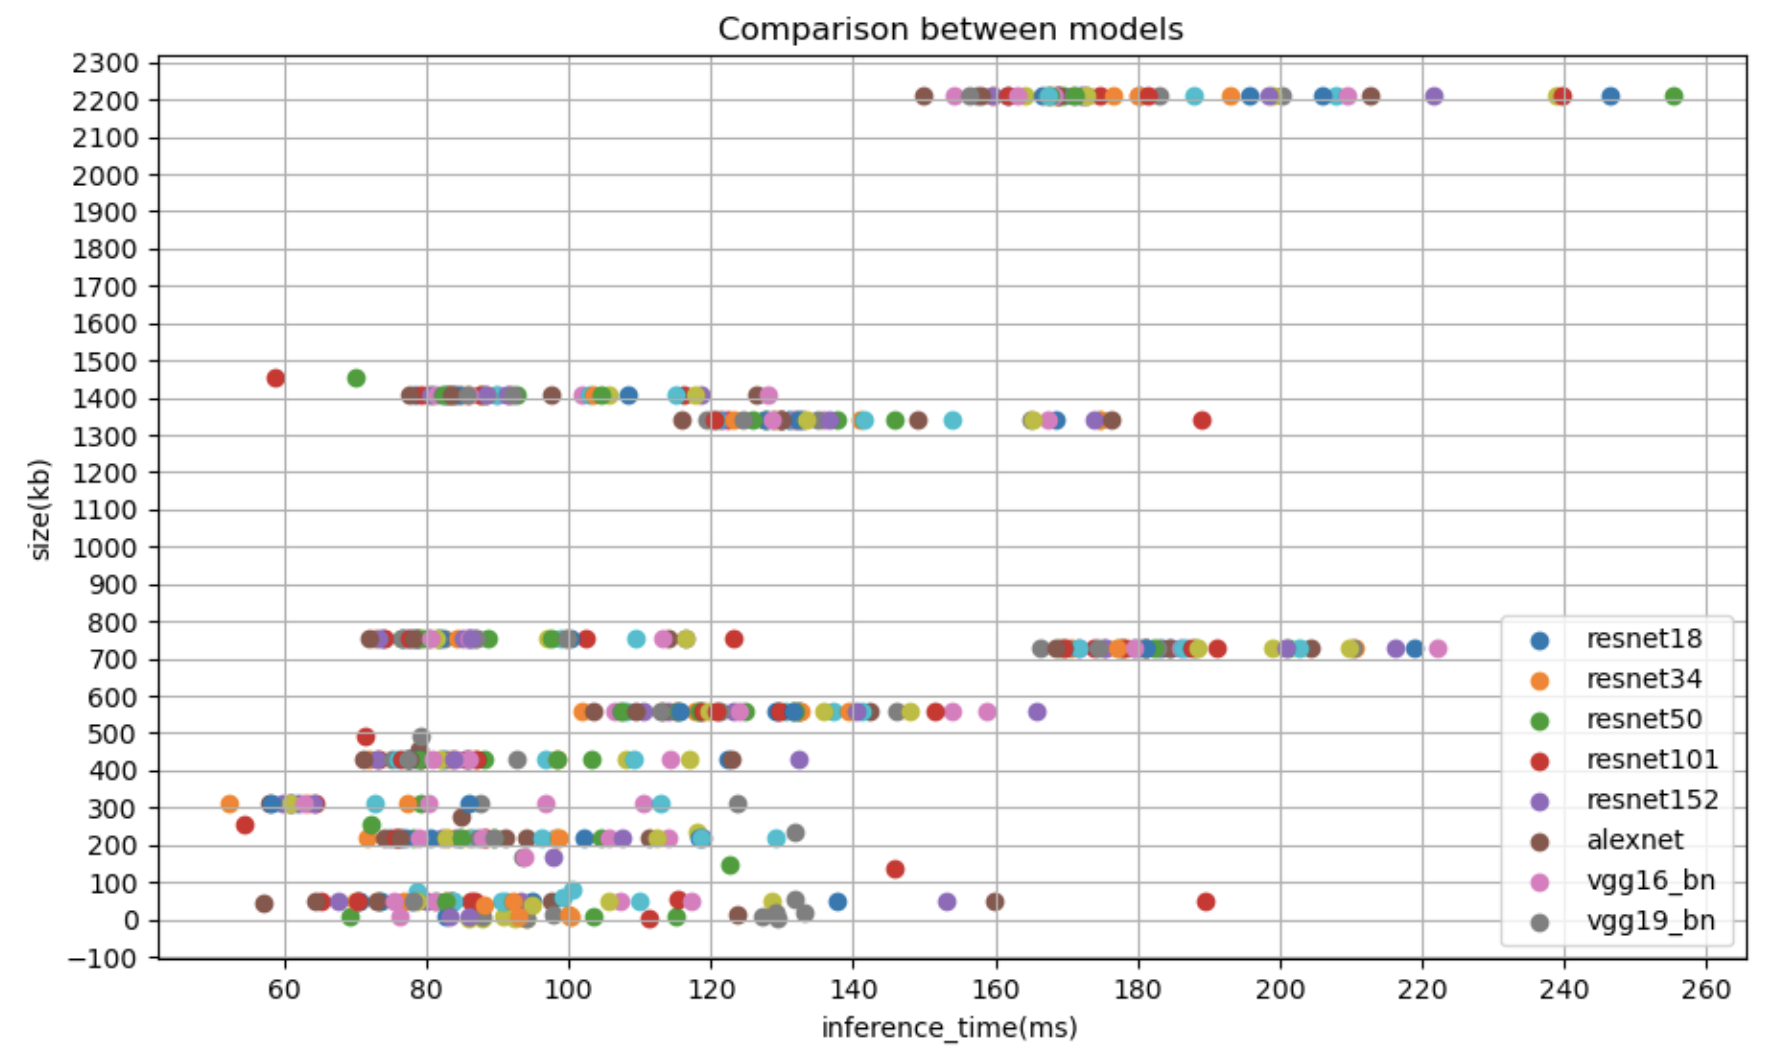
\includegraphics[width = 14 cm]{size_inference_time_compared.png}
        \caption[Size of the images over inference time]{This graph shows the size in kb of the ten slowest images over the time taken to be processed }
         \label{fig:size_inference_time_compared}
\end{figure}



From the graph we are able to spot some rather interesting behaviours. First of all, we would expect that for each epoch the slowest images would be the same. This hypothesis would be confirmed if the graph showed a group of pictures of the same size having different inference times. However, this is only the case for sizes bigger than 500 kbs. As a matter of fact, we are not able to cluster pictures before 500 kb under a certain inference time range as effectively as we can do for heavier pictures. We can conclude from this that regardless of the amount of training, pictures over 500kb are going to be the slowest ones. \\
From a closer investigation of the individual models emerged some differences in the response of the single models. \\
For deeper networks the situation is similar to the discussion we made. As shown in Fig. \ref{fig:sl_f_deep}, for both Resnet152 and VGG16, the response for pictures smaller than 500kb is noisy, although Resnet152 shows a more stable behaviour than VGG16. This implies that for these networks only the response with images over 500kb displays similarities.  
\begin{figure}[h]
     \begin{subfigure}{0.5\textwidth}
	    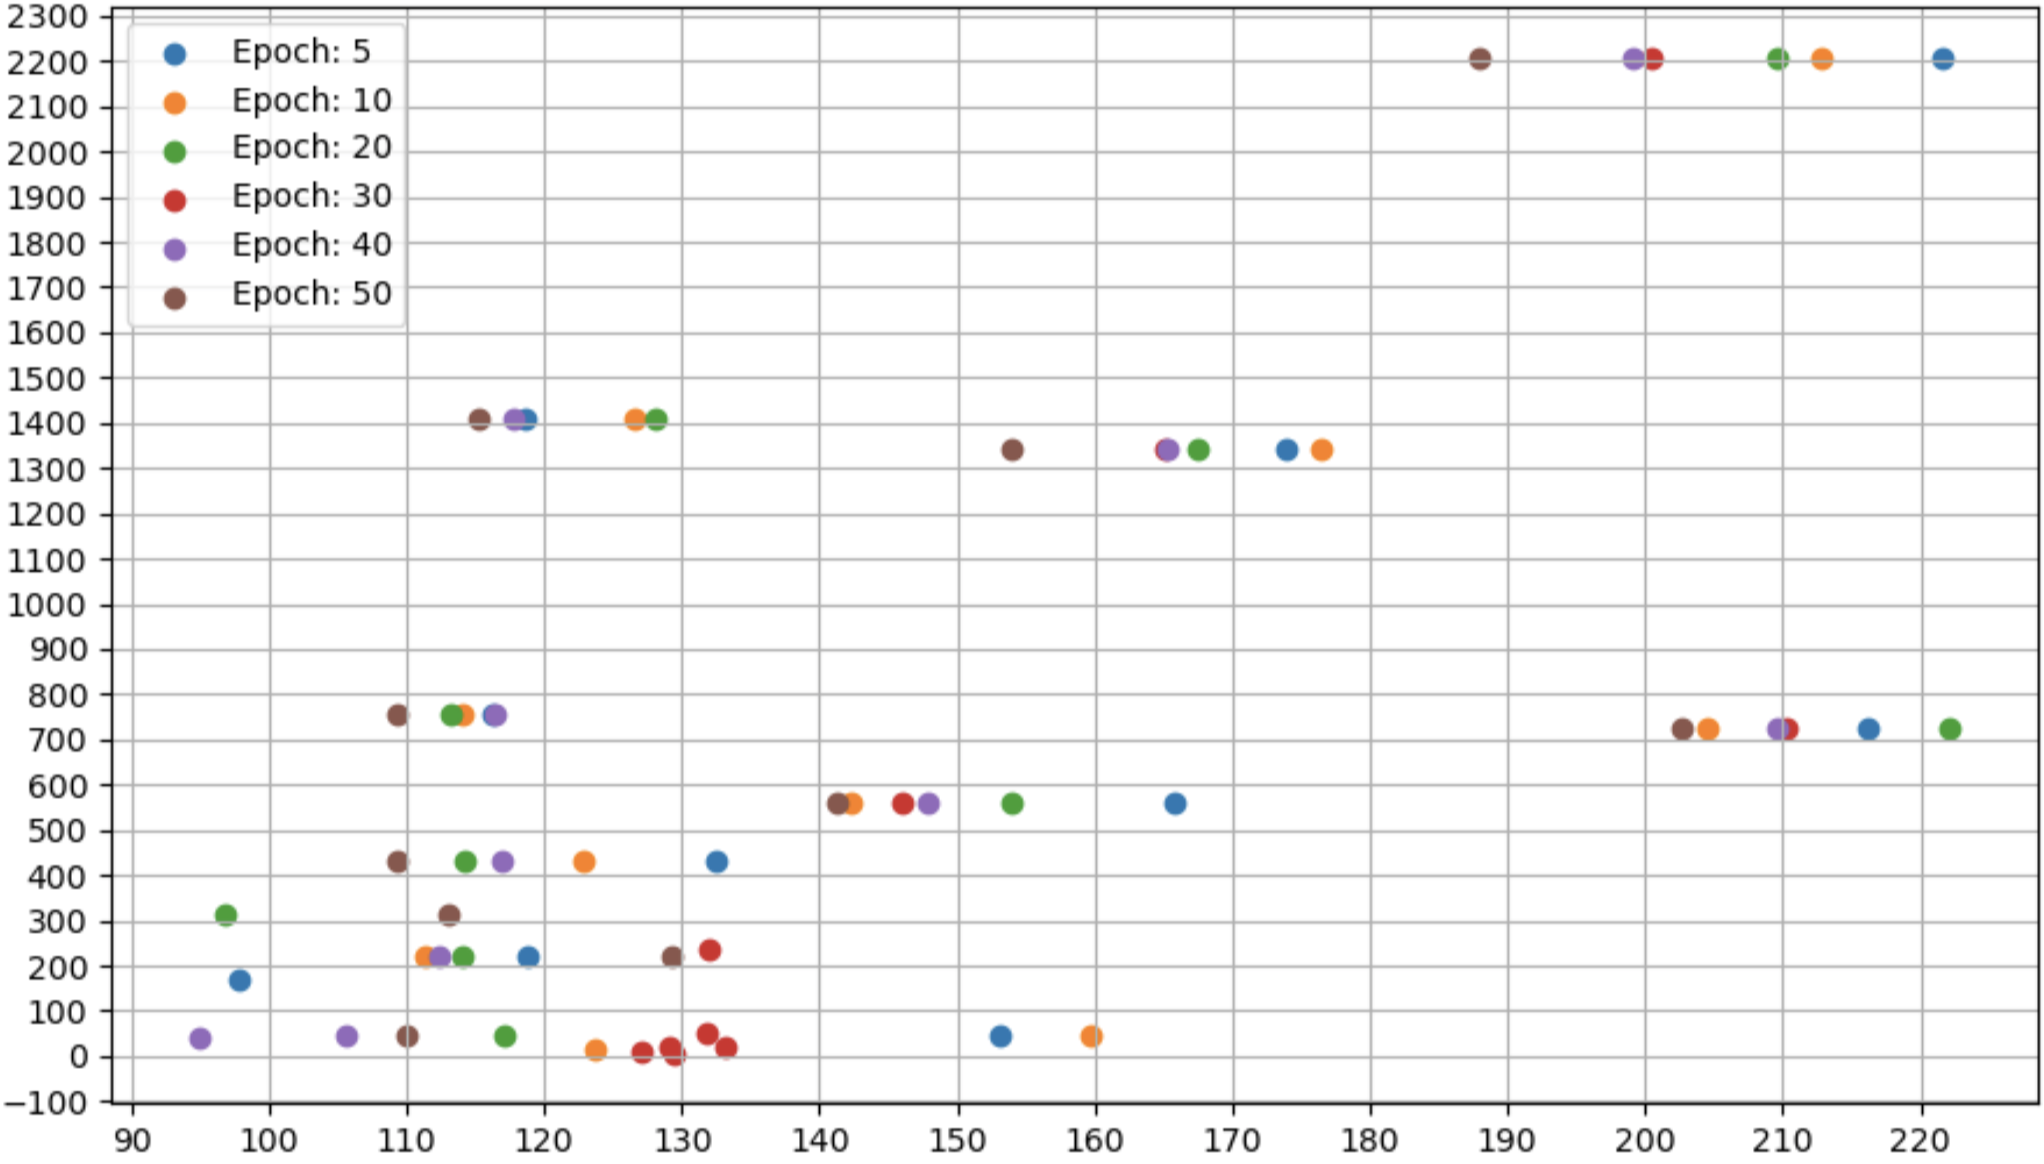
\includegraphics[width = \gws cm]{resnet152_sl_f.png}
	    \caption{Resnet152}
         \label{fig:resnet152_sl_f}
         
     \end{subfigure}
     \hfill
     \begin{subfigure}{0.5\textwidth}
	    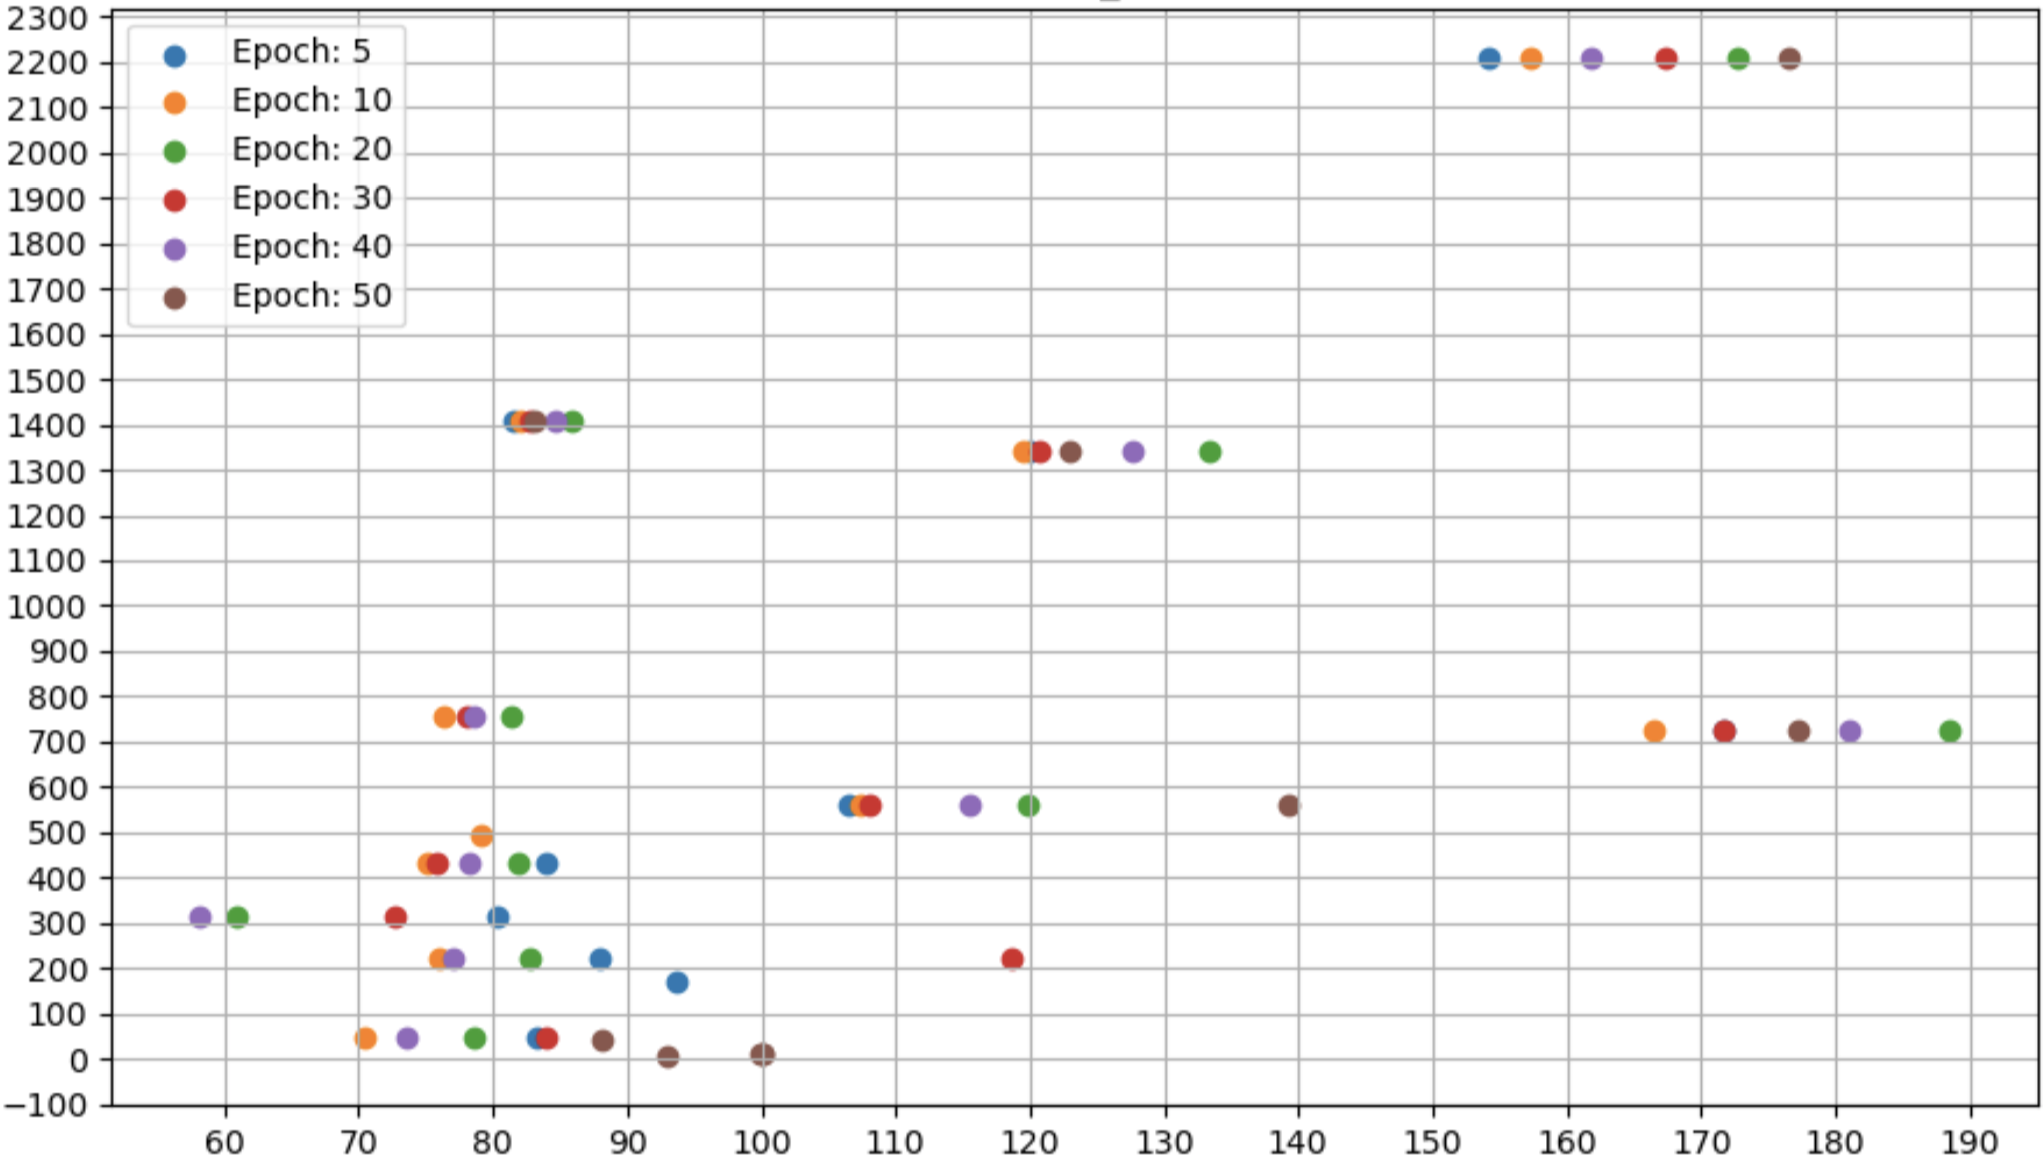
\includegraphics[width = \gws cm]{vgg16_sl_f.png}
	    \caption{VGG16}
        \label{fig:vgg16_sl_f}
        
     \end{subfigure}\\
     \caption{Inference time measured for model Resnet18 and Alexnet}
        \label{fig:sl_f_deep}
\end{figure}

For shallower networks, however, the situation is slightly more different. Fig. \ref{fig:sl_f_shallow} shows the slowest images identified in the models Resnet18 (Fig. \ref{fig:resnet18_sl_f}) and Alexnet (Fig. \ref{fig:alexnet_sl_f}). Differently from what we concluded before, these models show a much more precise response for images smaller than 500 kb. We are in fact able to cluster the images by size, with the exception of very few outliers. In addition, we can also point out which number of epochs would yield faster predictions for the slowest images. For Resnet18, we can observe that the model trained with 40 epochs is among the fastest for most sizes (with very few exceptions). For Alexnet, on the other hand, the fastest model is the one trained for only 10 epochs. This conclusion, however, does not take into account the accuracy that those models achieved. Using Fig. \ref{fig:inf_acc_resnet18} we can see that the same models, i.e. Resnet18 trained with 10 epochs, achieved one of the lowest accuracy rate overall (\textasciitilde90\%) and from Fig. \ref{fig:inf_acc_alexnet} we can extrapolate a similar conclusion for Alexnet trained with 10 epochs. (\textasciitilde80\%). \\
The best trade off between fast inference time and accuracy is achieved when both models have been trained with 50 epochs, however, in case of Resnet18, as we discussed before, this is also the number of epochs in which the validation loss is bigger than the training loss, hence we found ourselves in a situation of slight over-fitting. \\
\begin{figure}[h]
     \begin{subfigure}{0.5\textwidth}
	    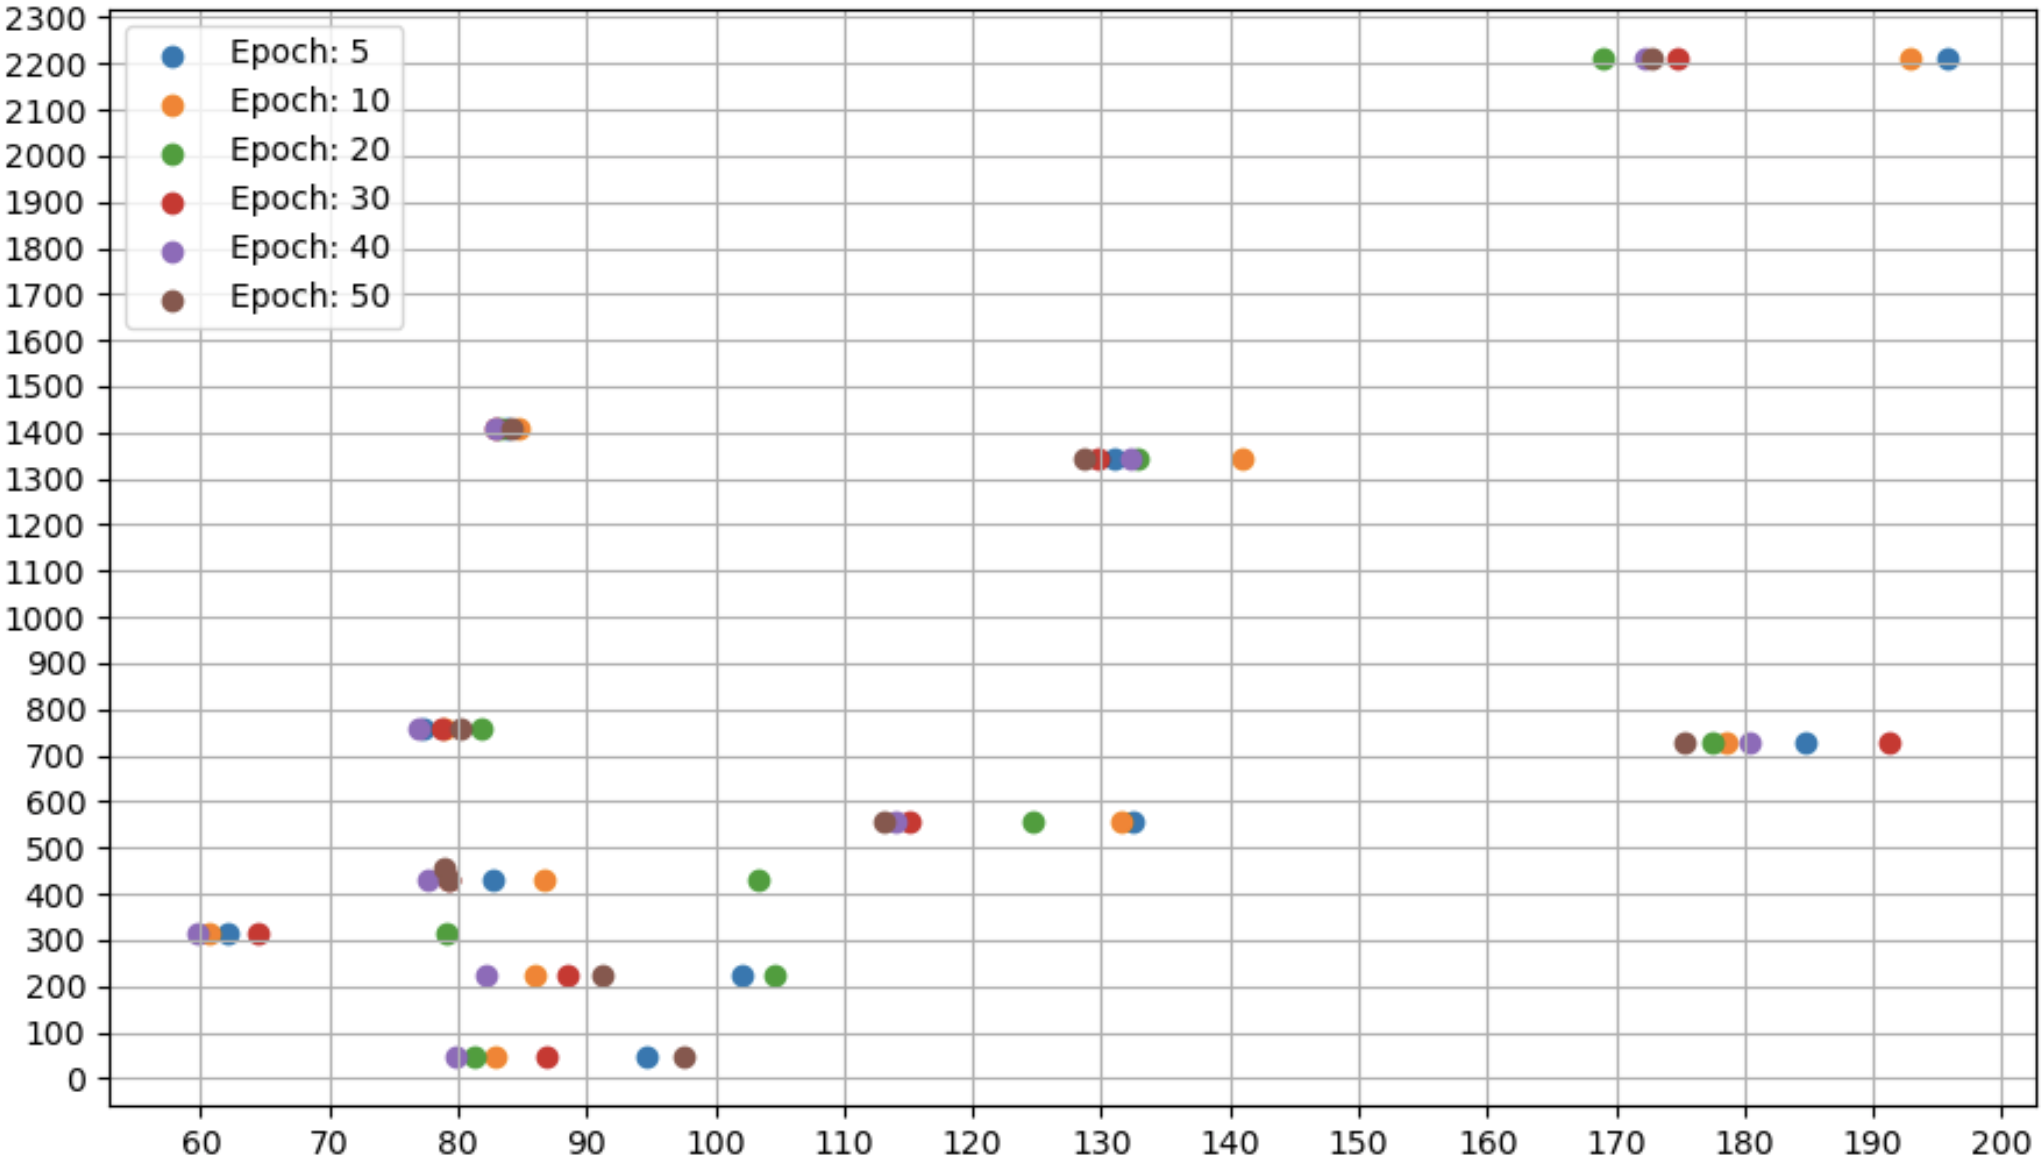
\includegraphics[width = \gws cm]{resnet18_sl_f.png}
	    \caption{Resnet18}
         \label{fig:resnet18_sl_f}
         
     \end{subfigure}
     \hfill
     \begin{subfigure}{0.5\textwidth}
	    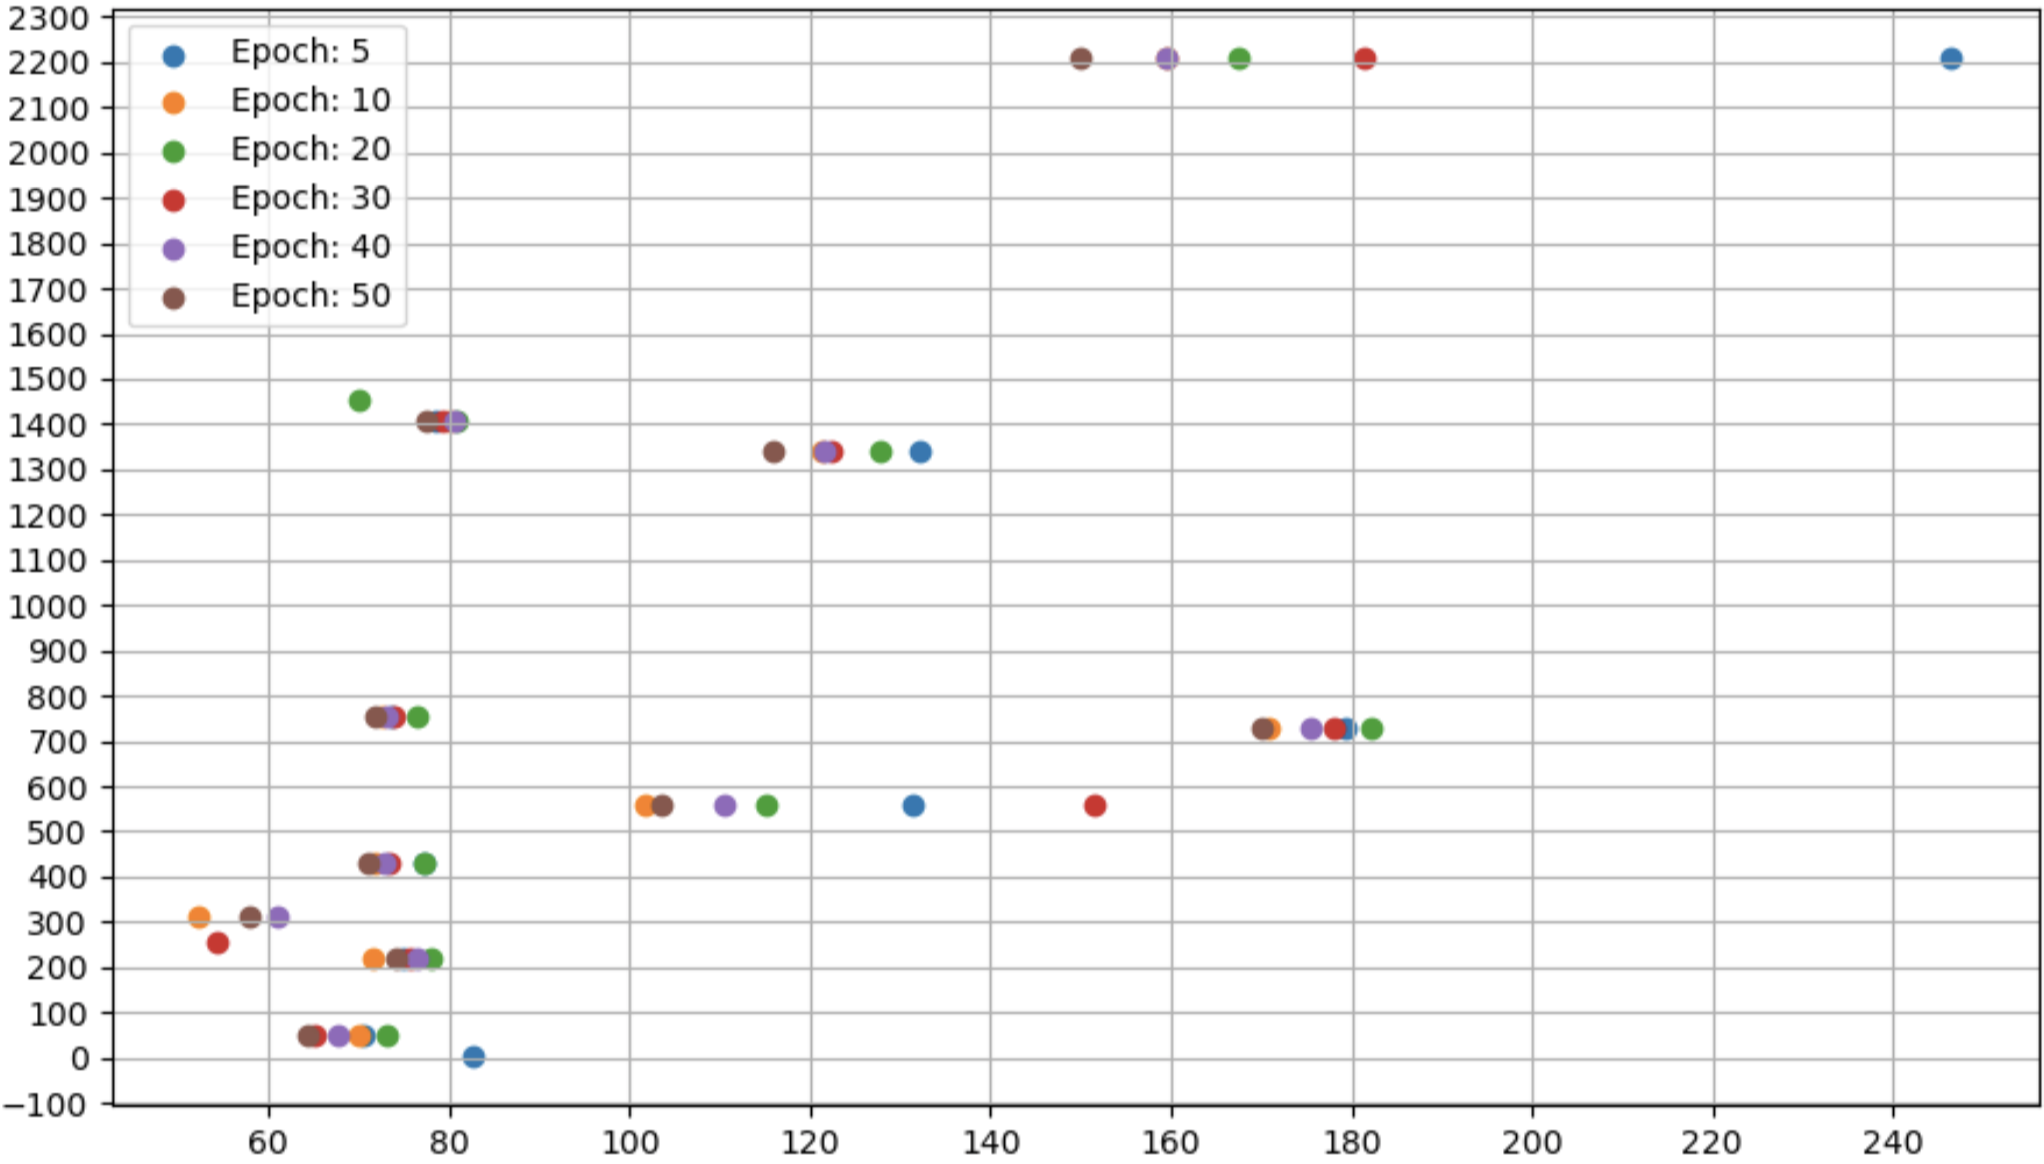
\includegraphics[width = \gws cm]{alexnet_sl_f.png}
	    \caption{Alexnet}
        \label{fig:alexnet_sl_f}
        
     \end{subfigure}\\
     \caption{Inference time measured for model Resnet18 and Alexnet}
        \label{fig:sl_f_shallow}
\end{figure}


Regardless of which number of epochs is better for this specific case, the purpose of our exploration is to identify correlation between certain characteristics. From these graphs we are able to find a correlation and to reason about it, in order to tailor future applications. \\
In a real world implementation, if it is known that images with a certain size are going to be among the slowest is useful because it will influence the decision of which hardware to mount on the devices sent to the fields. Additionally, knowing that images with a size of 700 kb are going to take from 200 to 220ms to be classified, will, naturally, help model the time behaviour of these devices and give information to verify that they will not miss any deadline. Furthermore, if we are able to reason about the trade-off between inference time and accuracy, we would also be able to choose a suitable model for different requirements. For example, in applications in which the system needs to respect a hard-deadline, inference time plays a more important role than overall accuracy. By being able to predict both inference time and accuracy from other characteristics, we can find a trade-off which will allow us to respect any hard-deadline. 


A closer look to the list of slowest images reveals that there are common pictures amongst all models (Fig. \ref{fig:slowest_files_all}). Using the tool we can investigate if those pictures present similarities that may explain why this is the case. The information collected from the pictures are shown in table 
\ref{tab:pictures_info}.

\begin{table}[htbp]
\centering
\begin{tabular}{ p{2cm} p{4cm}  p{2cm}  p{2cm}  }
 Picture n.& Dimensions(x,y) & DPI(x,y)&size(kb) \\
 \hline
1&(3888, 2187)&N/A& 727\\
2&(3018, 2585)&(300,300)&2209\\
3&(3000, 2019)&(300,300)&1341\\
4&(2003, 2003)&N/A&558\\
5&(1373, 1012)&(72,72)&1409\\
6&(2048, 1551)&(300, 300)&221\\
 \hline
\end{tabular}
\caption{Information collected from the slowest pictures}
\label{tab:pictures_info}
\end{table}

As already demonstrated by Fig. \ref{fig:size_inference_time_compared}, each of the five pictures has a size bigger than 500kb, i.e. they are amongst the heaviest pictures on the dataset. Furthermore, they are also amongst the pictures having the highest dimensions. Even though not available for all the pictures, table \ref{tab:pictures_info} also shows that the pictures have high DPI, which implies that these pictures have very high quality. \\
Following the calculations we delineated in section \ref{sec:ben_inf}, we can hypothesise that images with higher dimensions are more slowly processed by the models. This is due to the fact that each architecture presents pooling layers, which according to equation \ref{eq:Pl_FLOPS}, is directly proportional to the dimensions of the images. If we compare Fig. \ref{fig:size_inference_time_compared} and table \ref{tab:pictures_info}, we can also spot a quite interesting relation.
For example, if we analyse picture number 6, we can see that it has a size of 221 kb and dimensions of $2048 \times 1551$ pixels. According to our hypothesis, we would expect it to be slower than pictures having lower dimensions. However, picture 5, with dimension $1373 \times 1012$ pixels, is being processed more slowly or equally by every model at every epoch. We can therefore confute the hypothesis that we just made and conclude that the inference time is influenced not only by the dimension of the images, but also by other characteristics of the images. Studying and analysing these characteristics can produce further results that have not been considered in this paper. % lazy Luca


